\chapter{Results and Discussion}
\label{cap:resultados}

This chapter presents the results obtained from the analysis described in
Chapter \ref{cap:metodos}. They are revealed in the order in which the analysis
is built, starting by showing that the
selected jets and their substructure are described consistently in data and
simulation, followed by the results of the flavour labelling and
selection, and finally by the measurement of the spin-sensitive observables.

Section \ref{sec:res-kinematics} presents the selected jets and their kinematic
distributions. Section \ref{sec:res-lund} shows the primary and secondary Lund jet
planes, and Section \ref{sec:res-inclusive} the distribution of $\dpsi$ before any
flavour selection. Section \ref{sec:res-labelling} describes the composition of the
simulated sample in the channels defined by the IFN labelling and the modulation
associated with each of them. Section \ref{sec:res-performance} evaluates the
performance of the flavour selection and compares it with the alternative
approaches of Section \ref{sec:flavour-alternatives}. Section \ref{sec:res-modulation}
presents the central result of this work, the mean value
$\langle \cos 2\dpsi \rangle$ as a function of the threshold of the flavour
selection, in data and in simulation. Section \ref{sec:res-eeec} presents the
three-point energy correlator, and Section \ref{sec:res-discussion} discusses the
results in the light of the theoretical expectations and of the CMS measurement.

The achieved results were obtained at the level of reconstructed particles, and data
and simulation are compared at this same level. The collision data are those of the
JetHT dataset of Table~\ref{tab:dataset}, and the two simulation datasets are the
sample with $800 < \hat{p}_{\mathrm{T}} < 1000$~GeV, on which
the flavour selection is trained, and the sample with $600 < \hat{p}_{\mathrm{T}} < 800$~GeV 
which is used for the calibration of the purity
and for every comparison with data. The sample used in each figure is indicated in its
caption and, unless stated otherwise, the distributions shown are normalised to
unit area, so that their shapes are compared, and the uncertainties are
statistical only. The systematic uncertainties discussed in
Section~\ref{sec:systematic} are not represented in the figures.

\section{Event selection and jet kinematics}
\label{sec:res-kinematics}

The number of events and jets, of collision and simulation data, remaining after the selection of
Table~\ref{tab:selection} is shown in Table \ref{tab:jetcounts}. Of all the selected jets,
only those with primary and the secondary declustering contain a splitting satisfying $z > 0.1$ yield a valid
value of $\dpsi$. These jets define the sample on which all subsequent results are
based.

\begin{table}[htbp]
    \centering
    \caption{Number of events, selected jets and jets with a valid $\dpsi$, in the
    collision data and in the simulated calibration sample.}
    \label{tab:jetcounts}
    \begin{tabular}{lrrr}
      \toprule
      & Data & Simulation $600 < \hat{p}_{\mathrm{T}} < 800$ & Simulation $800 < \hat{p}_{\mathrm{T}} < 1000$ \\
      \midrule
      Events                     & 30 241 & 5 737 037 & 29 652 066 \\
      Selected jets              & 60 566 & 11 476 817 & 59 389 760 \\
      Jets with a valid $\dpsi$  & 45 755 & 8 495 207 & 43 071 113 \\
      \bottomrule
    \end{tabular}
\end{table}

The kinematic distributions of the selected jets are shown in Figure \ref{fig:jetpt},
for collision and simulation data. The three distributions start at $700$~GeV, because
of the imposed selection threshold. It is possible to see that in data, the distribution
falls smoothly and it extends to higher values, since it receives contributions from all intervals of
$\hat{p}_{\mathrm{T}}$. However, in simulation, the distributions fall much more quickly and
they struggle to reach the same higher values as in collision data, since their jets
originate from an interval of $600 < \hat{p}_{\mathrm{T}} < 800$~GeV
and $800 < \hat{p}_{\mathrm{T}} < 1000$~GeV. 
This difference is the one discussed in
Section \ref{sec:sys-purity}, and it should be kept in mind when comparing the
other distributions. Now, comparing the two simulated distribution it is worth noting that 
the $800 < \hat{p}_{\mathrm{T}} < 1000$~GeV distribution extends further above the selection threshold.
Although the flavour selection is trained, calibrated and 
applied on jets with partly different distributions, the measurement is still possible since 
the jet transverse momentum is excluded from its inputs, as discussed in
Section~\ref{sec:flavour-features}, while
the residual effect of this difference on the purity is discussed in
Section~\ref{sec:sys-purity}.

\begin{figure}[htbp]
  \centering
  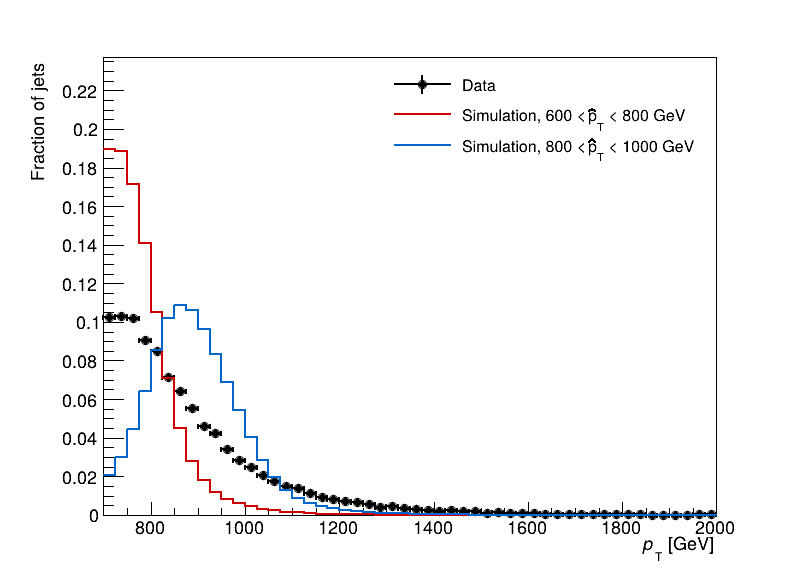
\includegraphics[width=0.6\textwidth]{figuras/jetpt_jets.png}
  \caption{Transverse-momentum distribution of the selected jets in the collision
  data and in the simulated samples with $600 < \hat{p}_{\mathrm{T}} < 800$~GeV and
  $800 < \hat{p}_{\mathrm{T}} < 1000$~GeV, normalised to unit area.}
  \label{fig:jetpt}
\end{figure}

The other distribution which is relevant for the comparison of the different
datasets is the number of constituents of the selected jets. This is the extracted
quantity most related to the substructure observables, since it shows 
the amount of radiation inside a jet, and it contributes to the flavour selection
procedure through the
multiplicities of the branches of the second splitting.
Its distribution is shown
in Figure~\ref{fig:nconst} for the collision data and for the two simulated
samples, normalised to unit area. The three distributions are very similar,
peaking at about $35$ constituents and extending up to about $130$. The simulated
samples reproduce the shape of the data very closely.

\begin{figure}[htbp]
  \centering
  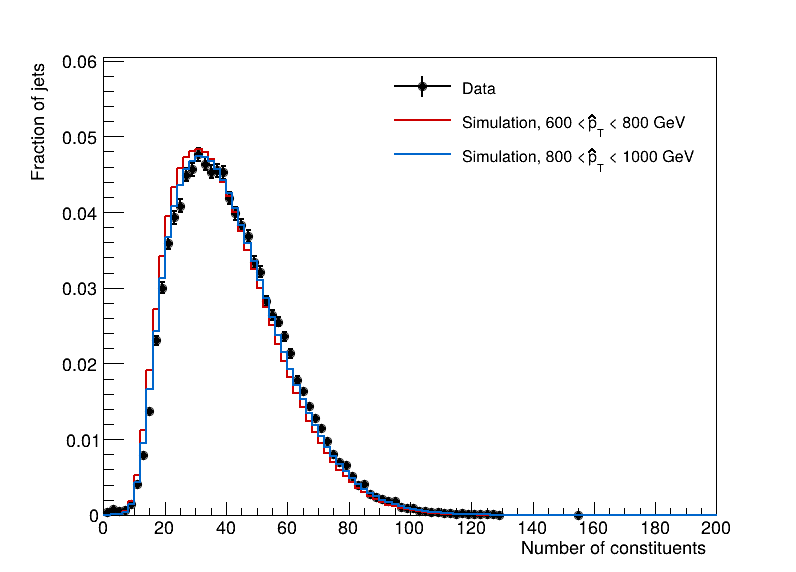
\includegraphics[width=0.6\textwidth]{figuras/nconst_jets.png}
  \caption{Number of constituents of the selected jets in the collision data and
  in the simulated samples with $600 < \hat{p}_{\mathrm{T}} < 800$~GeV and
  $800 < \hat{p}_{\mathrm{T}} < 1000$~GeV, normalised to unit area.}
  \label{fig:nconst}
\end{figure}

The very small difference between the samples represent well the pattern from their 
transverse momenta. The sample with $600 < \hat{p}_{\mathrm{T}} < 800$~GeV,
whose jets are the softest, is slightly shifted towards lower number of
constituents while the sample with $800 < \hat{p}_{\mathrm{T}} < 1000$~GeV lies closest to the
data. This difference is very small despite the very different spectra of Figure~\ref{fig:jetpt},
reflecting a slow growth of the number of constituents with the jet's transverse momentum.
The data lies slightly above both simulated samples between $50$ and $80$ constituents,
which may reflect the modelling of the
parton shower and of hadronisation, as well as differences in the pile-up
conditions between data and simulation, since neutral pile-up particles remain
among the constituents. Nevertheless, the number of constituents of the jets is 
well described by the simulation. Since the multiplicities of the branches are among the inputs of the
flavour selection, this agreement supports, although it does not by itself
establish, the transfer of the selection from simulation to data discussed in
Section~\ref{sec:sys-purity}.

\section{Lund jet planes}
\label{sec:res-lund}

The average primary and secondary Lund planes obtained from the collision and simulated calibration samples respectively,
are shown in Figure \ref{fig:lund-planes}. Each plane shows the density $\rho$ of equation \eqref{eq:lund-density},
which is the number of emissions per jet and per unit area in
the coordinates $\ln(1/\dR)$ and $\ln \kt$. Since the observable $\dpsi$ is the final measurement
of this work, only the declusterings that satisfy the condition $z > 0.1$ are included.

The shape of the populated region follows from the definition of section \ref{sec:ca}.
Since $\kt = z\,(p_{\mathrm{T},a} + p_{\mathrm{T},b})\,\dR$,
the emissions of a given branch with fixed momentum fraction lie on straight lines
of slope $-1$ in the plane,

\begin{equation}
  \ln \kt = \ln z + \ln\!\left( p_{\mathrm{T},a} + p_{\mathrm{T},b} \right)
            - \ln\frac{1}{\dR} .
  \label{eq:lund-zlines}
\end{equation}

The upper edge of the plane corresponds to the limit of $z=1/2$, because it is the largest
momentum fraction allowed when the softer branch is taken as the emission, and the
condition $z > 0.1$ imposes a parallel lower edge. Therefore, for a parent with
fixed momentum, the emissions should occupy a diagonal band of width $\ln 5$ in $\ln \kt$
at fixed angle. However, in practice, the momentum of a parent varies along the
declustering sequence and from jet to jet, which broadens the band and smooths its
edges. The left side of the plane is bounded by the radius of the jets, because the jet's 
widest splittings seperate two subjets whose axes lie within the jet, so that their
separation rarely exceeds $R = 0.8$, corresponding to $\ln(1/\dR) \approx 0.2$.

In primary Lund plane, the density along the band is approximately 
uniform at large angles and large transverse momenta, at about $0.2$ emissions per jet and per
unit area which is the expected behaviour in the perturbative region from Section \ref{sec:lund-uniform}.
In addition, towards smaller angles the density raises, reaching its maximum 
around $\ln(1/\dR) \approx 4.5$ and $\ln \kt \approx 0$, that
is for $\kt$ of order $1$~GeV, and then falling at lower transverse momenta. 
This maximum lies where $\kt$ approaches the scale of hadronisation, and marks the
transition to the non-perturbative region of the plane.

The secondary Lund plane is populated by emissions of the softer branch of the primary splitting,
but it shows the same properties. However, since this branch carries only a fraction of
momentum of the jet, the band is shifted towards lower transverse momenta, 
by about one unit in $\ln \kt$, and it is broader, as this fraction varies
from jet to jet and its maximum lies at larger angles than in the primary plane,
at around $\ln(1/\dR) \approx 3.3$. This comes from equation \eqref{eq:lund-zlines}, where
a branch with lower momentum has the region of $\kt \approx 1$~GeV, where the density peaks,
at a larger angular separation.

\begin{figure}[htbp]
  \centering
  \begin{subfigure}[b]{0.49\textwidth}
    \centering
    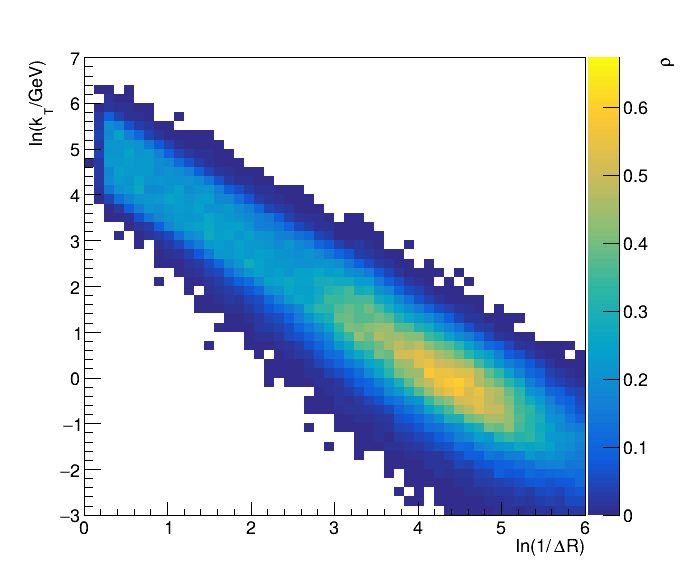
\includegraphics[width=\textwidth]{figuras/lund_primary_data.png}
    \caption{Primary plane, data.}
  \end{subfigure}
  \hfill
  \begin{subfigure}[b]{0.49\textwidth}
    \centering
    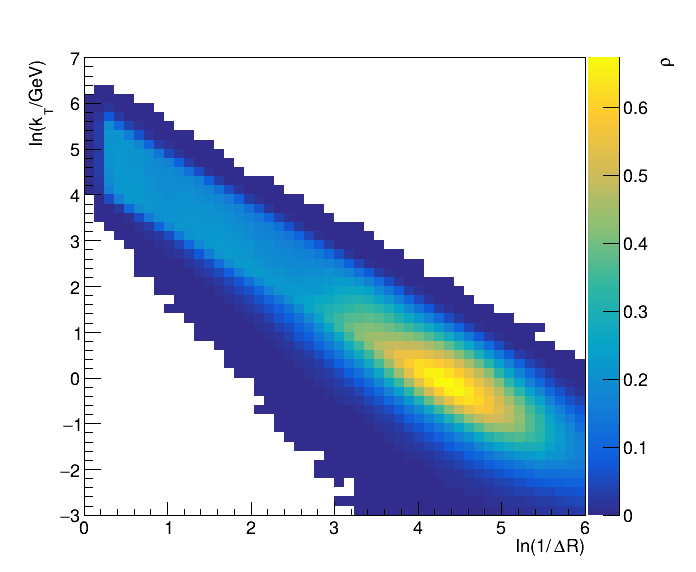
\includegraphics[width=\textwidth]{figuras/lund_primary_sim.png}
    \caption{Primary plane, simulation.}
  \end{subfigure}
  \\[6pt]
  \begin{subfigure}[b]{0.49\textwidth}
    \centering
    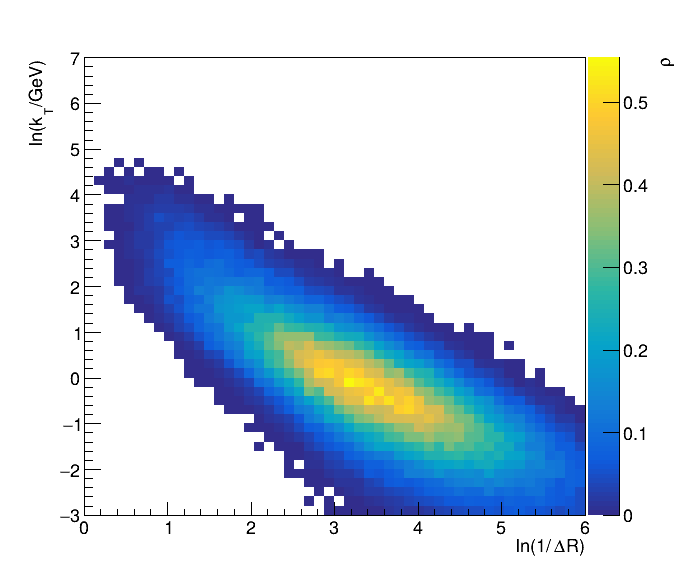
\includegraphics[width=\textwidth]{figuras/lund_secondary_data.png}
    \caption{Secondary plane, data.}
  \end{subfigure}
  \hfill
  \begin{subfigure}[b]{0.49\textwidth}
    \centering
    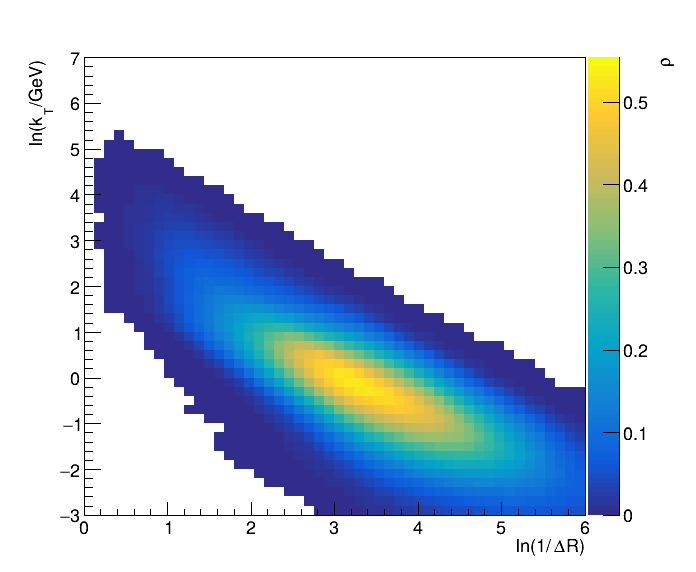
\includegraphics[width=\textwidth]{figuras/lund_secondary_sim.png}
    \caption{Secondary plane, simulation.}
  \end{subfigure}
  \caption{Average primary (top) and secondary (bottom) Lund jet planes of the jets
  with a valid $\dpsi$, in the collision data (left) and in the simulated sample
  with $600 < \hat{p}_{\mathrm{T}} < 800$~GeV (right). Only declusterings
  satisfying $z > 0.1$ are included. The colour scale shows the density of
  emissions per jet and per unit area, with the same scale for data and simulation
  in each row.}
  \label{fig:lund-planes}
\end{figure}

Now, comparing the collision data to the simulation, it is notable that they have a very close
structure. The position and
extent of the bands, and the location of their maxima, agree between data and
simulation within the precision of the maps, which
for the data show larger fluctuations owing to their smaller number of jets.
This similarity shows that the reconstruction and declustering of the jets behave
consistently in data and simulation. This also involves the quantities $z$,
$\kt$ and $\dR$ of the selected splittings, which enter the flavour selection as
inputs, and thus supports the use of the selection trained in simulation on
the collision data.

\section{Inclusive \texorpdfstring{$\dpsi$}{Delta psi 12} distribution}
\label{sec:res-inclusive}

The obtained distribution of $\dpsi$ for all jets with a valid value, before any
flavour selection, is shown in Figure \ref{fig:dpsi-inclusive} for the collision data and
for the simulated calibration sample. With the convention of equation \eqref{eq:dpsi-impl},
the angle is defined in the range of $[0,\pi]$, over which
$\cos 2\dpsi$ completes one full period. In this figure it is notable that the form of 
equation \eqref{eq:dpsi-modulation} has a negative coefficient $a_2/a_0$ with an excess 
of jets around $\dpsi = \pi/2$, where the two splitting planes are
perpendicular, and a depletion near $\dpsi = 0$ and $\pi$, where they are aligned.

\begin{figure}[htbp]
  \centering
  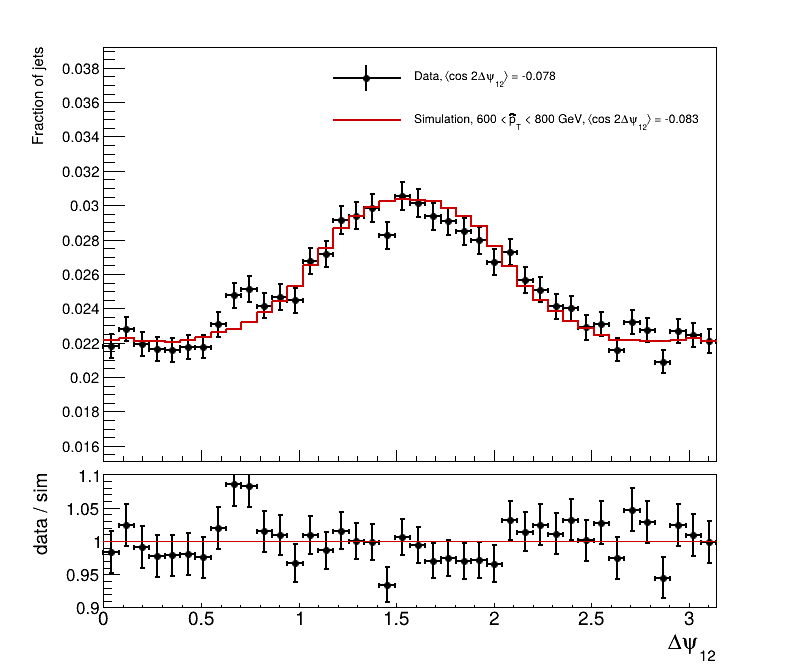
\includegraphics[width=0.7\textwidth]{figuras/dpsi_inclusive.png}
  \caption{Distribution of $\dpsi$ for all jets with a valid value, before any
  flavour selection, in the collision data and in the simulated sample with
  $600 < \hat{p}_{\mathrm{T}} < 800$~GeV, normalised to unit area.}
  \label{fig:dpsi-inclusive}
\end{figure}

The distribution shows a clear modulation of this kind. The fraction of jets rises
from about $0.022$ per bin near $\dpsi = 0$ and $\pi$ to about $0.030$ around
$\pi/2$. The mean values are

\begin{equation}
  \langle \cos 2\dpsi \rangle_{\text{data}} = -0.0780 \pm 0.0033 ,
  \qquad
  \langle \cos 2\dpsi \rangle_{\text{sim}} = -0.0831 \pm 0.0002 ,
  \label{eq:inclusive-values}
\end{equation}

where the uncertainties are statistical. Through the relation
$a_2/a_0 = 2\langle \cos 2\dpsi \rangle$, they correspond to coefficients of
$-0.156 \pm 0.007$ and $-0.166 \pm 0.001$ respectively. The two values differ by
about $1.5$ standard deviations, and the simulation describes the shape of the
distribution in data within about $5\%$ in almost every bin, the few larger
deviations being compatible with statistical fluctuations. However, the shape is not
of a pure $\cos 2\dpsi$ modulation since the distribution is nearly flat close to 
$\dpsi = 0$ and $\pi$, and its central maximum is narrower than of a single harmonic modulation, 
which may indicate the presence of higher harmonics in addition to the
$\cos 2\dpsi$ term.

This inclusive result is dominated by splittings that are unmatched or belong to channels
other than $g \to q\bar{q}$, as shown in Table~\ref{tab:composition}. Therefore, this modulation
is a superposition of all contributions of different channels and it is diluted according to it.
Thus, this distribution serves as baseline for evaluating the impact of the flavour selection 
in Section~\ref{sec:res-performance}, while the significance of its magnitude is examined in Section~\ref{sec:res-modulation}.

\section{Channel labelling}
\label{sec:res-labelling}

The composition of the simulated training sample in the channels defined by the
IFN labelling of Section~\ref{sec:genlevel} is given in
Table~\ref{tab:composition} while for the simulated calibration sample is given by
the following Table~\ref{tab:cos2-labels}. The composition obtained also agrees closely with 
the one obtained in the
CMS measurement with \textsc{Pythia}~8, the same flavour definition and the same
matching of the branches $p_3$ and $p_4$, namely $72\%$, $16\%$, $8\%$, $3\%$ and
$1\%$~\cite{CMS:2026jnt}. The agreement confirms that the labelling was constructed 
correctly, although it does not prove whether the
simulation describes the data.

The mean value $\langle \cos 2\dpsi \rangle$ obtained from the simulated 
calibration sample is also given in Table~\ref{tab:cos2-labels},
together with the value predicted at second
order in the collinear limit for the corresponding channel~\cite{Karlberg_2021}.
This prediction was computed on electron-positron collisions without hadronisation
or detector effects, and, in this work, it serves only as a reference point for the sign 
and the order of magnitude of each contribution

\begin{table}[htbp]
  \centering
  \caption{Mean value $\langle \cos 2\dpsi \rangle$ for the jets of each channel of
  the IFN labelling, in the simulated calibration sample, with statistical
  uncertainties. The last column gives the prediction of
  Ref.~\cite{Karlberg_2021} for the corresponding channel, obtained for
  electron-positron collisions with $z_1, z_2 > 0.1$.}
  \label{tab:cos2-labels}
  \begin{tabular}{lrrrr}
    \toprule
    Class & Jets & Fraction (\%) & $\langle \cos 2\dpsi \rangle$ & Prediction \\
    \midrule
    $g \to q\bar{q}$   & $179\,810$     & $3.1\%$  & $-0.167 \pm 0.002$ & $-0.31$ \\
    $g \to gg$         & $857\,140$     & $14.7\%$ & $-0.077 \pm 0.001$ & $+0.025$ \\
    $q \to qg$         & $358\,498$     & $6.1\%$  & $-0.091 \pm 0.001$ & $0$ \\
    unmatched          & $4\,397\,983$  & $75.2\%$ & $-0.0585 \pm 0.0003$ & --- \\
    rest               & $53\,911$      & $0.9\%$  & $-0.161 \pm 0.003$ & --- \\
    \midrule
    all labelled jets  & $5\,847\,342$  & $100\%$ & $-0.0674 \pm 0.0003$ & ---\\
    \bottomrule
  \end{tabular}
\end{table}

The $g \to q\bar{q}$ channel shows a modulation with $\langle \cos 2\dpsi \rangle = -0.167 \pm 0.002$,
while the $q \to qg$ and $g \to gg$ channels, which form the background of the flavour selection, give
together $-0.081 \pm 0.001$. Thus, the modulation of the $g \to q\bar{q}$ channel is
about twice as strong as that of the background, and it is this
difference that the flavour selection exploits. In Figure~\ref{fig:qq_vs_all}, it is possible to see
the difference between the $g \to q\bar{q}$ channel and the whole sample. It is important 
to note that the sign of the $g \to q\bar{q}$ class agrees with the prediction, while its magnitude
is smaller which is expected for a flavour based label that does not coincide splitting by splitting with the channel
of the parton shower and for an observable built from reconstructed particles. More importantly,
the $q \to qg$ and $g \to gg$ classes also show a negative sign in contrast with 
the vanishing and slightly positive values predicted for the
corresponding channels. A negative contribution is thus present in every class,
including those in which no spin correlation is expected and its source is discussed
in Section~\ref{sec:res-discussion}.

\begin{figure}[htbp]
  \centering
  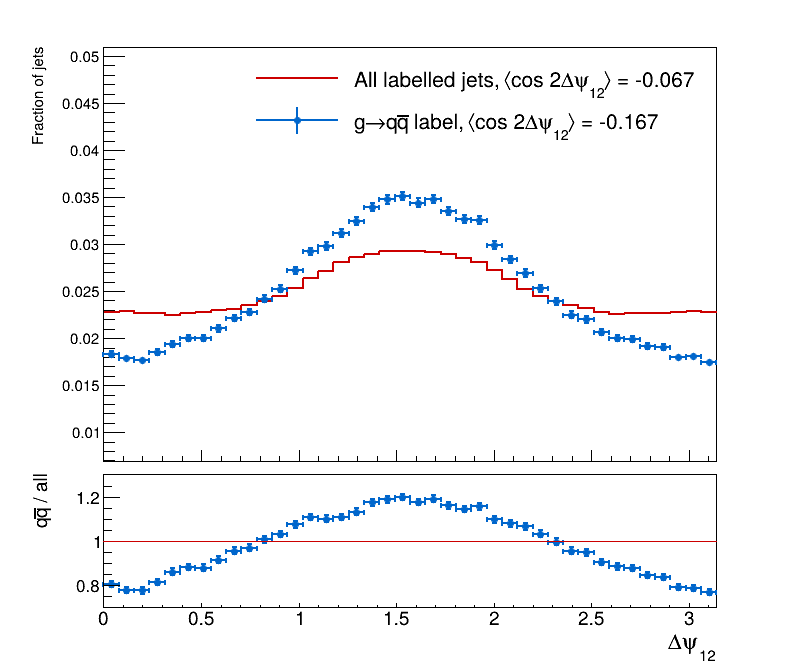
\includegraphics[width=0.7\textwidth]{figuras/dpsi_labels.png}
  \caption{Distribution of $\dpsi$ for all labelled jets and for the jets whose
  second splitting is labelled $g \to q\bar{q}$, in the simulated sample with
  $600 < \hat{p}_{\mathrm{T}} < 800$~GeV, normalised to unit area. The lower
  panel shows the ratio of the $g \to q\bar{q}$ distribution to that of all
  labelled jets.}
  \label{fig:qq_vs_all}
\end{figure}

\subsection{Momentum fractions of the two splittings}
\label{sec:res-zplane}

The momentum fractions $z_1$ and $z_2$ of the primary and secondary selected splittings
are two of the features used by the flavour selection of
Section~\ref{sec:flavour}. Each is the fraction carried by the softer branch and lies
between the SoftDrop grooming condition of $z = 0.1$ and $z = 1/2$. Their complete
distribution is shown in Figure \ref{fig:zplane-channels} for all jets with a valid 
$\dpsi$, in data and in simulation, and for the simulated jets in each channel.
The ratio of each distribution to that of all simulated jets is shown in
Figure~\ref{fig:zplane-ratios}, where the differences between the channels can be 
distinguished more easily.

\begin{figure}[htbp]
  \centering
  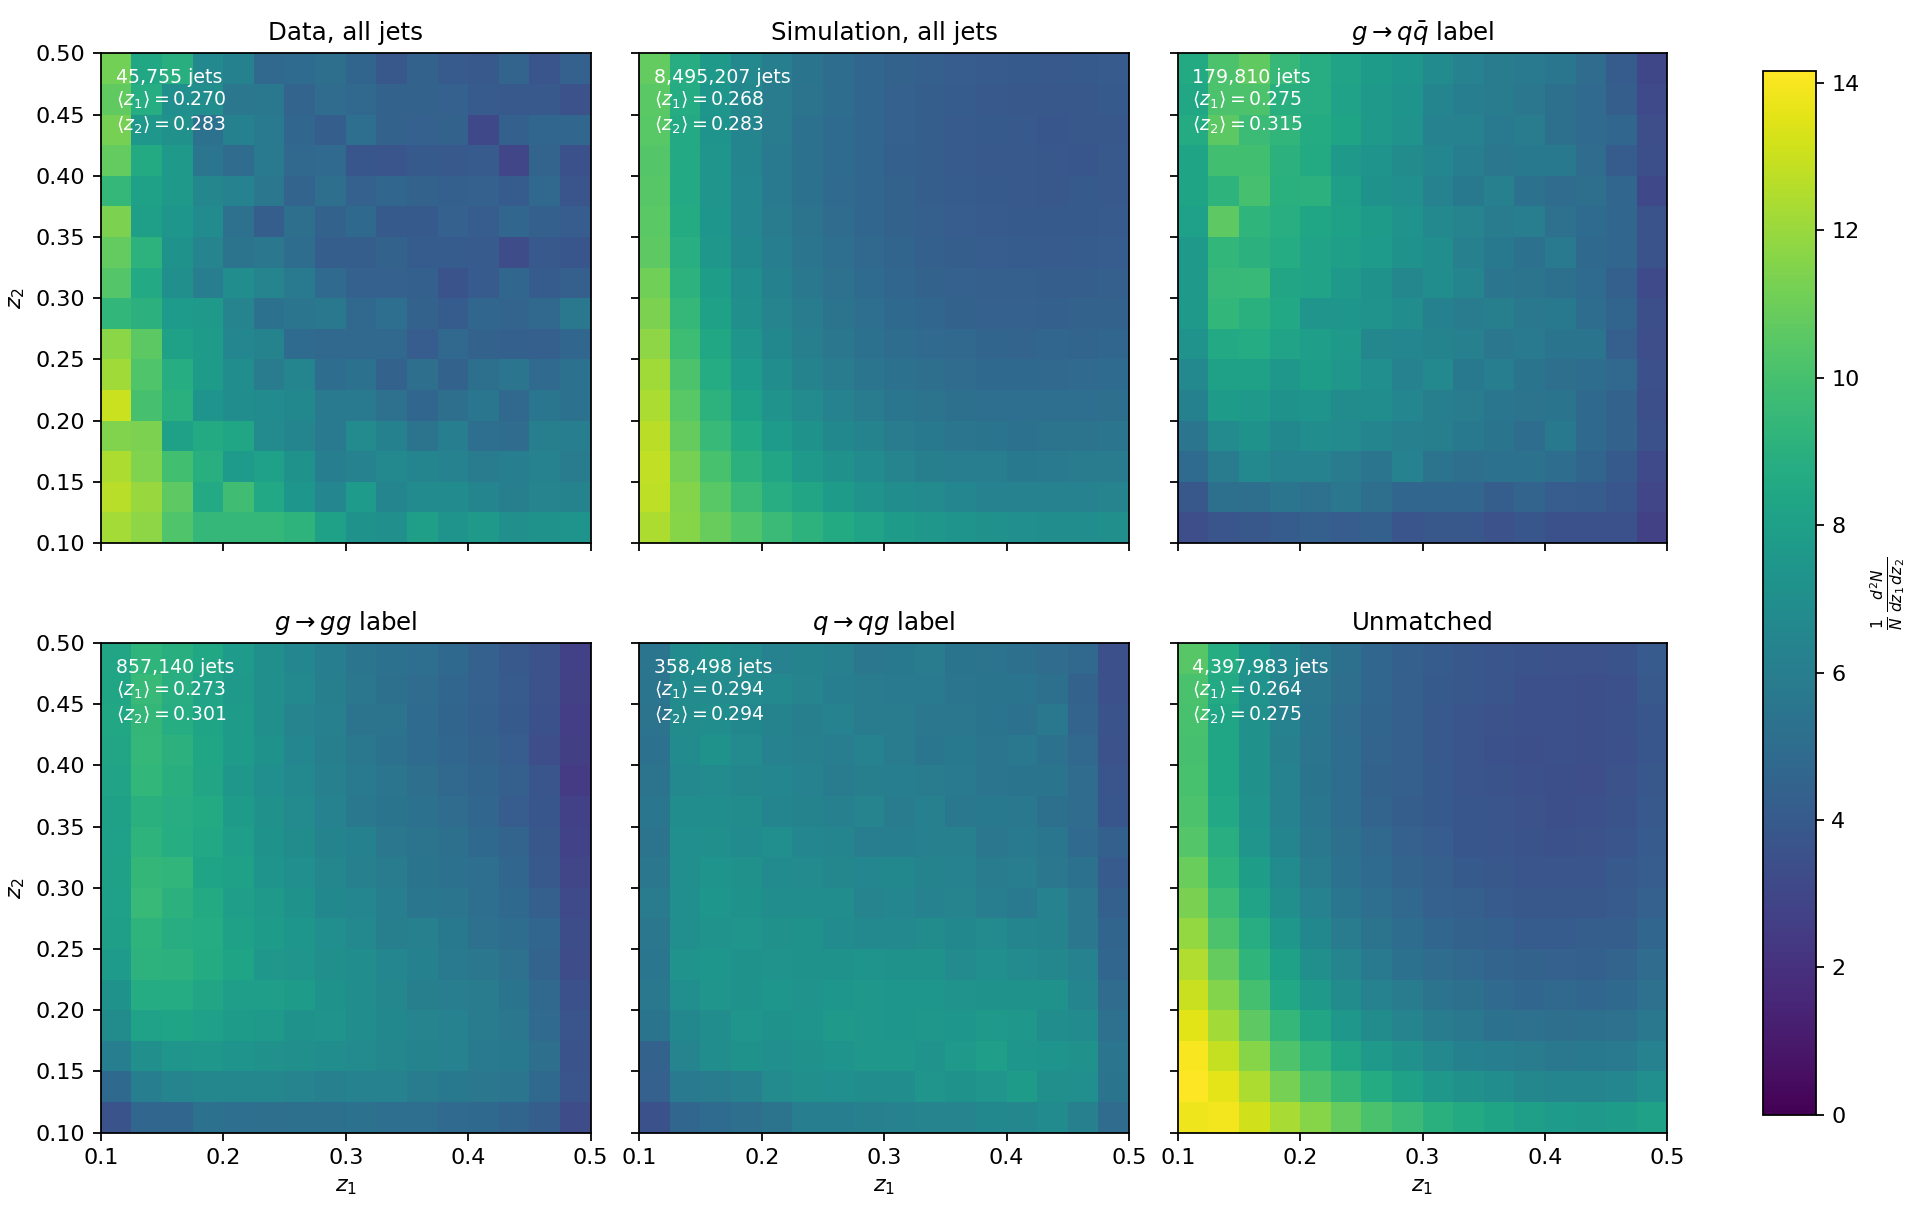
\includegraphics[width=\textwidth]{figuras/zplane_channels.png}
  \caption{Distribution of the momentum fractions $z_1$ and $z_2$ of the first and
  second selected splittings, normalised to unit area, for all jets with a valid
  $\dpsi$ in the collision data and in the simulated calibration sample, and for
  the simulated jets labelled $g \to q\bar{q}$, $g \to gg$ and $q \to qg$ and
  those unmatched. Each panel gives the number of jets and the mean values of
  $z_1$ and $z_2$.}
  \label{fig:zplane-channels}
\end{figure}

\begin{figure}[htbp]
  \centering
  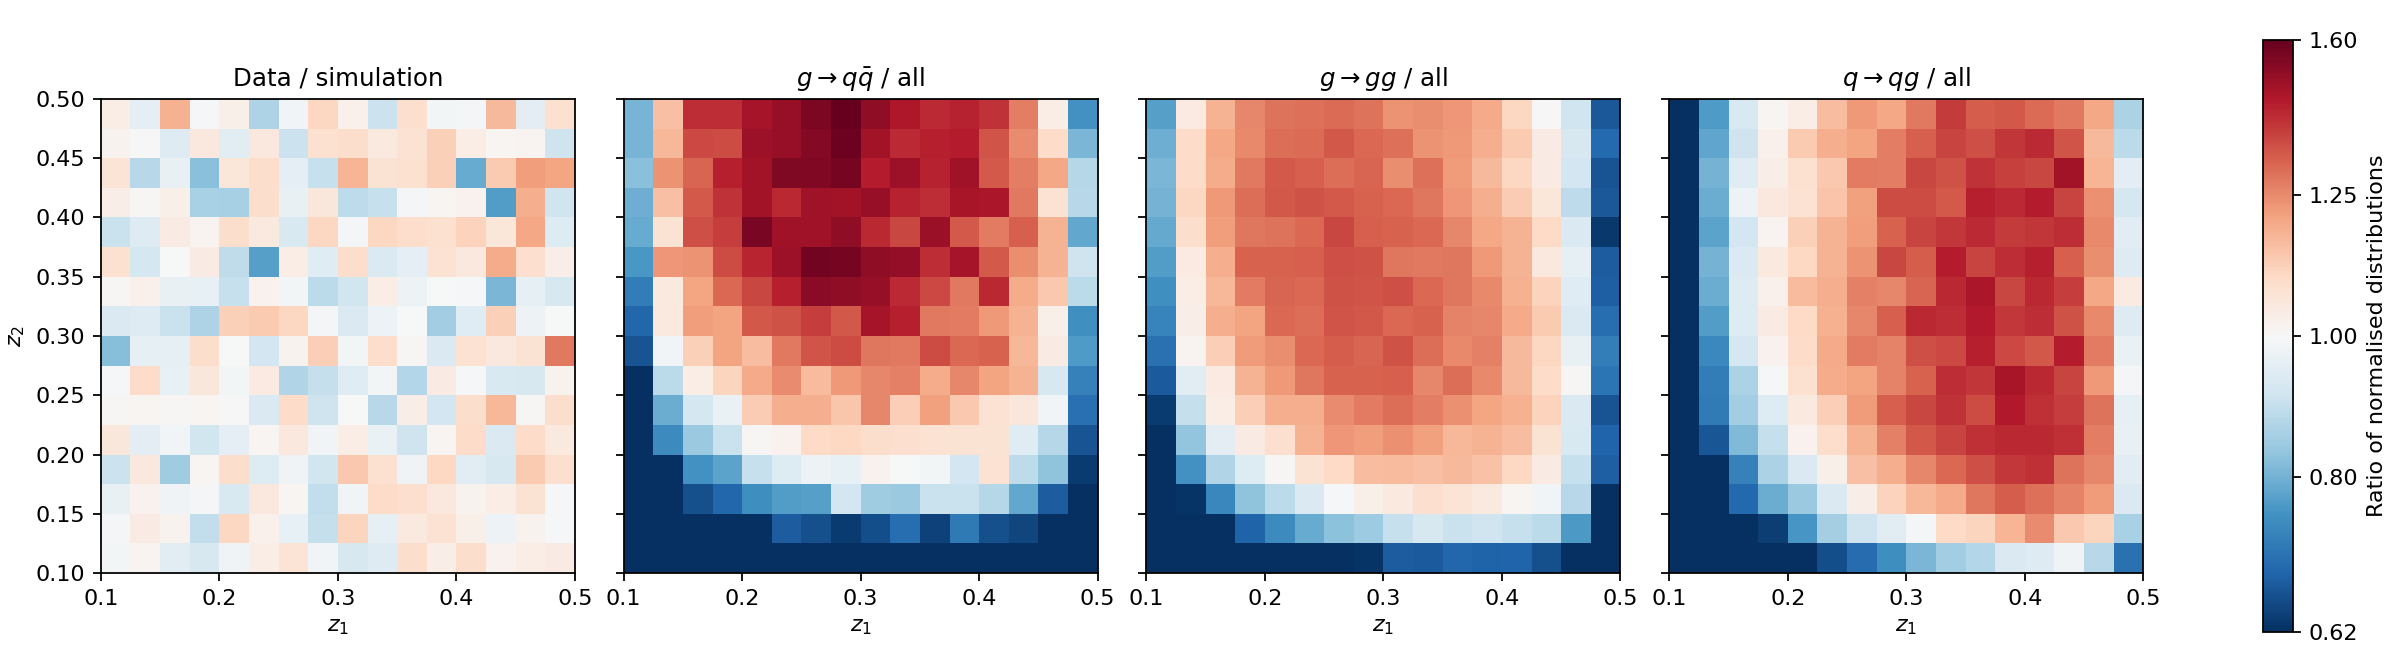
\includegraphics[width=\textwidth]{figuras/zplane_ratios.png}
  \caption{Ratio of the normalised distributions of
  Figure~\ref{fig:zplane-channels} to that of all simulated jets, for the
  collision data and for the simulated jets labelled $g \to q\bar{q}$, $g \to gg$
  and $q \to qg$. The colour scale is logarithmic and symmetric around unity, and
  ratios beyond its range are shown at its limits.}
  \label{fig:zplane-ratios}
\end{figure}

The distribution of all jets is concentrated at small $z_1$ and $z_2$, so that asymmetric splittings
with soft branch dominate the sample. The simulation describes the collision data well
with mean values of $\langle z_1 \rangle = 0.270$ and $\langle z_2 \rangle = 0.283$ in data, against
$0.268$ and $0.283$ in simulation, and the ratio of the two distributions shows no
systematic structure, only fluctuations compatible with the statistical
precision of the data.

The channels populate the plane differently. The unmatched jets, which make up
about half of the sample, are concentrated in the corner of small $z_1$ and $z_2$,
with $\langle z_1 \rangle = 0.264$ and $\langle z_2 \rangle = 0.275$. Soft branches
are the most affected by hadronisation and by the detector, so their splittings
are the least often matched at generator level. The labelled channels instead
populate the interior of the plane. The jets labelled $g \to q\bar{q}$ have the
largest $\langle z_2 \rangle$, $0.315$. Relative to all jets they are enhanced by
$50\%$ or more for $0.3 \lesssim z_2 \lesssim 0.45$ and intermediate $z_1$, and
suppressed by more than a third for $z_2 < 0.15$. This reflects the splitting
function of Eq.~\eqref{eq:Pgq}, which has no enhancement for soft splittings,
in contrast with those of $g \to gg$ and $q \to qg$. The jets labelled $g \to gg$
show a similar but weaker pattern, with $\langle z_2 \rangle = 0.301$. The jets
labelled $q \to qg$ differ mainly in $z_1$, with the largest mean value,
$\langle z_1 \rangle = 0.294$, and an enhancement at $z_1 \gtrsim 0.3$.
For the second splitting to be $q \to qg$, the softer branch of the first splitting must
be a quark, and a quark is produced without the soft enhancement associated with
an emitted gluon. Therefore, the first splitting of these jets is more symmetric.

As one can notice, all channels have a depletion near the edge of $z_1 \to 1/2$.
When the primary splitting is nearly symmetric, its softer branch is decided by small
differences in the transverse momentum of the splitting's daughters. So, 
the generator-level and the reconstructed declusterings can then follow different
branches to the secondary splitting, making the algorithm label the secondary 
splitting as unmatched.

These differences are the information in $z_1$ and $z_2$ that the flavour
selection can exploit. The $g \to q\bar{q}$ channel is distinguished mainly by
its more symmetric second splitting, and the effect of the selection on the
distribution of $z_2$ is examined in Section~\ref{sec:res-mod-z}.

\section{Flavour selection performance}
\label{sec:res-performance}

In order to measure the spin-sensitive observable using the flavour selection, discussed
in Section \ref{sec:flavour}, it must first be shown that it can identify the $g \to q\bar{q}$ channel
effectively. This section evaluates its performance in simulation, where the IFN
label of every splitting is known, and compares it with the alternative approaches
of Section~\ref{sec:flavour-alternatives}.

As stated before, two simulated samples were used, for different purposes. 
The separation achieved by
each network is assessed on the test subset of the training sample, with
$800 < \hat{p}_{\mathrm{T}} < 1000$~GeV, which was not used during the training.
It is characterised by the distributions of the scores for the different channels
and by the area under the ROC curve, which measures the ability of the network to
rank a splitting of the signal channels above one of the background. For the second
stage, in which the $g \to q\bar{q}$ channel is a minority, the area under the
precision-recall curve is also given, since it reflects more directly the purity
that can be achieved. The performance of the complete selection, expressed through
the purity and the efficiency of equation \eqref{eq:purity-efficiency}, is determined
instead on the independent calibration sample, with
$600 < \hat{p}_{\mathrm{T}} < 800$~GeV. This is the sample on which the purity of
the measurement is calibrated, and it allows all methods to be compared without
any bias from their training.

Section~\ref{sec:res-twostage} presents the performance of the two stages of the
selection and the purity reached as a function of the threshold.
Section~\ref{sec:res-alternatives} compares the two-stage selection with the
alternative approaches.

\subsection{Two-stage selection}
\label{sec:res-twostage}

The first stage network separates matched from unmatched splittings performing it with an area
under the ROC curve of $0.840$, as shown in Figure~\ref{fig:roc-stage1}. This network 
performance is sufficient in order to remove the majority number of unmatched secondary
splittings before the flavour of the second splitting is examined. In Figure~\ref{fig:confusion},
the confusion matrix of the first stage classifier, obtained from the test subset, is shown.
Since unmatched splittings form the bulk of the data sample, a classifier trained on this imbalance
could assign almost all splittings to this class. The matrix presented reveals that this is 
not the case. The results revealed that of the unmatched splittings, $87.4\%$ are correctly identified and $12.6\%$ are
classified as matched, while $61.8\%$ of the matched splittings are correctly
identified and $38.2\%$ are classified as unmatched. Therefore, both classes were
recognised as intended by the class weights during training. However, since the
unmatched splittings are about three times more numerous, the $12.6\%$
of them classified as matched still make up about $40\%$ of all the splittings
assigned to the matched class. This is why the matched score is set to be above
$0.8$, rather than the assignment to the most probable class on which the matrix is based.

\begin{figure}[htbp]
  \centering
  \begin{subfigure}[b]{0.49\textwidth}
    \centering
    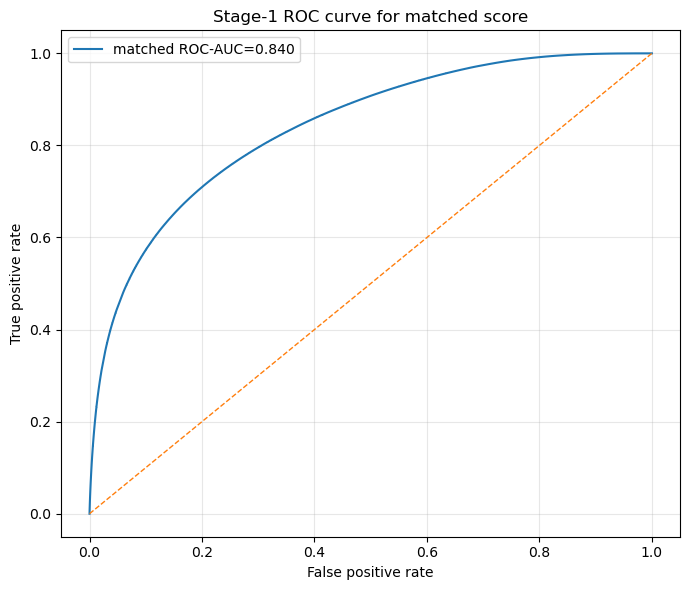
\includegraphics[width=\textwidth]{figuras/roc_stage1.png}
    \caption{ROC curve.}
    \label{fig:roc-stage1}
  \end{subfigure}
  \hfill
  \begin{subfigure}[b]{0.49\textwidth}
    \centering
    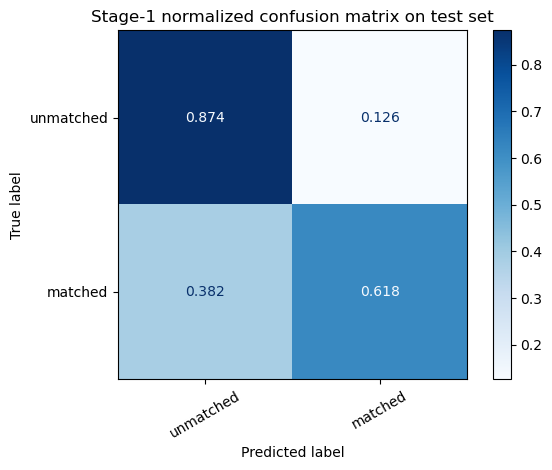
\includegraphics[width=\textwidth]{figuras/confusion.png}
    \caption{Confusion matrix.}
    \label{fig:confusion}
  \end{subfigure}
  \caption{Performance of the first stage on the test subset of the simulated
  sample with $800 < \hat{p}_{\mathrm{T}} < 1000$~GeV. (a) ROC curve of the matched
  score. (b) Confusion matrix, in which each row is normalised to the number of
  splittings of the corresponding true class and each splitting is assigned to
  the class of highest probability.}
  \label{fig:stage1-performance}
\end{figure}

The performance of the second stage is evaluated on the population 
on which it was trained which are the splittings labelled as $g \to q\bar{q}$, $q \to qg$ or $g \to gg$.
The distribution of its score for the $g \to q\bar{q}$ class and for the other two
classes together is shown in Figure~\ref{fig:score-stage2}. Both distributions
peak at about $0.3$, and the background is concentrated in the range between $0.2$ and $0.4$.
The main and most important difference between these two distributions is that the 
$g \to q\bar{q}$ class has a long tail extending to scores of about $0.65$, in which it dominates.
These scores are although confined between $0.15$ and $0.7$, which reflects the strong overlap
of the channels in the space of the input features and the use of the focal loss,
which does not push the outputs towards the extreme values.

\begin{figure}[htbp]
  \centering
  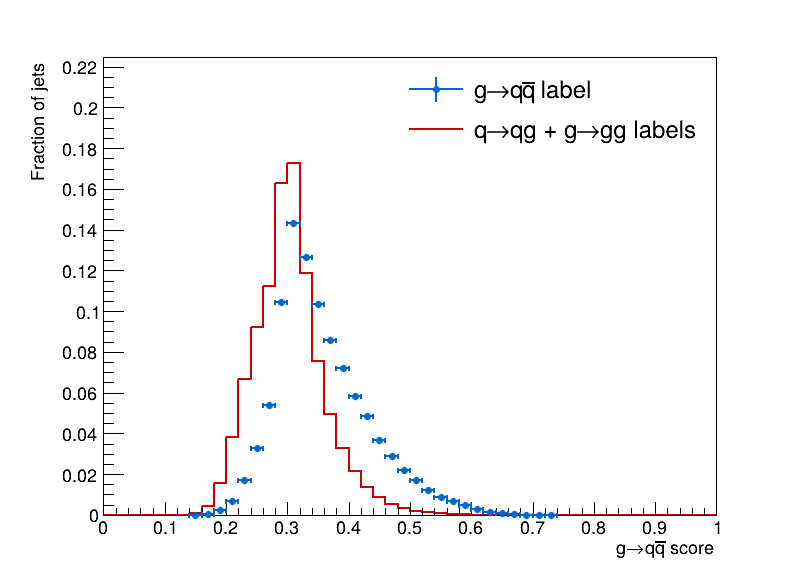
\includegraphics[width=0.7\textwidth]{figuras/score_stage2.png}
  \caption{Distribution of the $g \to q\bar{q}$ score of the second stage for the
  $g \to q\bar{q}$ class and for the $q \to qg$ and $g \to gg$ classes together, on
  the simulated calibration sample with $600 < \hat{p}_{\mathrm{T}} < 800$~GeV,
  normalised to unit area.}
  \label{fig:score-stage2}
\end{figure}

The ROC and precision-recall curves are shown in Figure~\ref{fig:roc-pr-stage2}.
The area under the ROC curve is $0.714$, which is worse compared to the first stage classifier, and the
area under the precision-recall curve is $0.314$, compared with $0.129$ for a
classifier without discriminating power, which corresponds to the fraction of the
$g \to q\bar{q}$ class among the matched splittings. The same areas were computed 
on the simulated calibration sample and the values of $0.715$ and $0.314$ were obtained for the 
ROC and precision-recall curves respectively. These values show that this network generalises 
to jets outside its training sample and the precision-recall curve also shows 
that a high purity is reached only at a small
efficiency, the purity exceeding $0.6$ only for efficiencies below about $10\%$.

\begin{figure}[htbp]
  \centering
  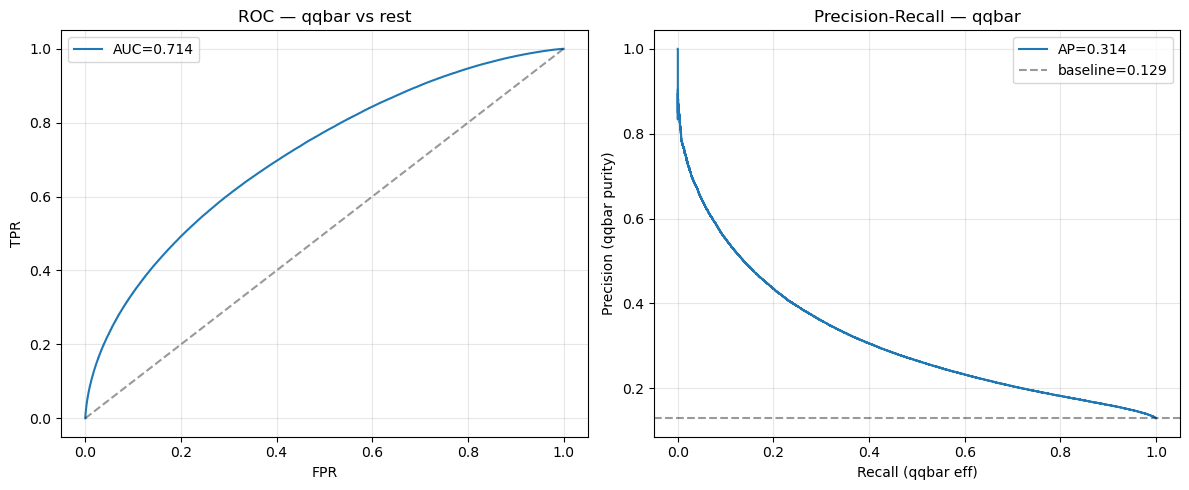
\includegraphics[width=\textwidth]{figuras/roc_pr_stage2.png}
  \caption{ROC curve (left) and precision-recall curve (right) of the
  $g \to q\bar{q}$ score of the second stage. The dashed line in the right panel
  shows the precision of a classifier without discriminating power.}
  \label{fig:roc-pr-stage2}
\end{figure}

The purity and the efficiency of the second stage on the test sample are
given in Table~\ref{tab:purity-threshold} and shown in
Figure~\ref{fig:purity-efficiency-threshold} as a function of the threshold.
As the threshold increases from $0.30$ to $0.60$, the purity rises steadily from
$0.18$ to $0.80$, while the efficiency falls from $81\%$ to below $1\%$. Above
$0.60$ the purity continues to rise, but the number of selected jets falls to a
few hundred and then even less, meaning that these thresholds carry little statistical
weight.

\begin{table}[htbp]
  \centering
  \caption{Number of selected jets, purity and efficiency of the second stage as a
  function of the threshold on the $g \to q\bar{q}$ score, for the splittings
  labelled $g \to q\bar{q}$, $q \to qg$ or $g \to gg$ in the simulated calibration
  sample with $600 < \hat{p}_{\mathrm{T}} < 800$~GeV. The uncertainties on the
  purity are statistical, and the efficiency is relative to all splittings
  labelled $g \to q\bar{q}$.}
  \label{tab:purity-threshold}
  \begin{tabular}{rrcr}
    \toprule
    Threshold & Selected jets & Purity & Efficiency (\%) \\
    \midrule
    $0.30$ & $1\,319\,798$ & $0.1807 \pm 0.0003$ & $80.6$ \\
    $0.35$ & $534\,802$    & $0.270 \pm 0.001$ & $48.7$ \\
    $0.40$ & $211\,459$    & $0.379 \pm 0.001$ & $27.1$ \\
    $0.45$ & $81\,911$     & $0.500 \pm 0.002$ & $13.8$ \\
    $0.50$ & $30\,446$     & $0.616 \pm 0.003$ & $6.3$ \\
    $0.55$ & $10\,111$     & $0.716 \pm 0.005$ & $2.5$ \\
    $0.60$ & $2\,455$      & $0.802 \pm 0.008$ & $0.67$ \\
    $0.65$ & $319$         & $0.865 \pm 0.019$ & $0.09$ \\
    $0.70$ & $16$          & $0.94 \pm 0.06$   & $0.01$ \\
    \bottomrule
  \end{tabular}
\end{table}

\begin{figure}[htbp]
  \centering
  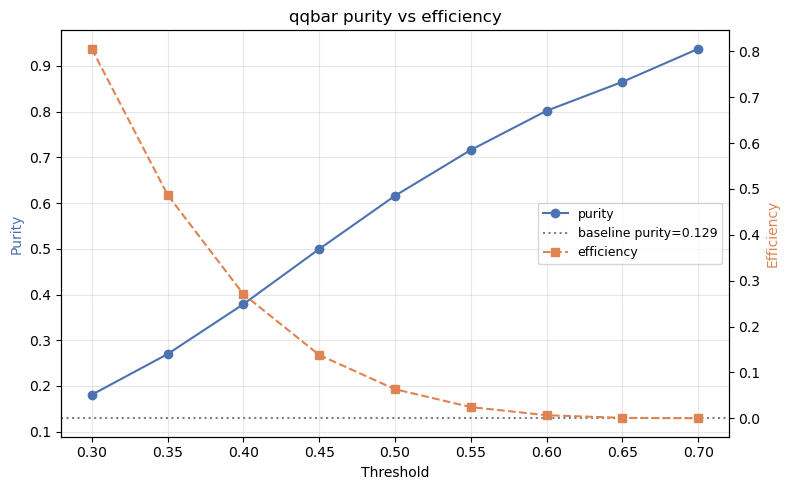
\includegraphics[width=0.75\textwidth]{figuras/purity_efficiency.png}
  \caption{Purity (left axis) and efficiency (right axis) of the second stage as a
  function of the threshold on the $g \to q\bar{q}$ score, for the splittings
  labelled $g \to q\bar{q}$, $q \to qg$ or $g \to gg$ in the simulated calibration
  sample. The dotted line shows the fraction of $g \to q\bar{q}$ splittings among
  these, before any selection.}
  \label{fig:purity-efficiency-threshold}
\end{figure}

\subsection{Comparison with alternative approaches}
\label{sec:res-alternatives}

The three alternative approaches of Section~\ref{sec:flavour-alternatives} are compared with the
previous two-stage selection on the simulated calibration sample. A first comparison
was made regarding the performance of the networks, evaluated on the splittings labelled as
$g \to q\bar{q}$, $q \to qg$ or $g \to gg$. On this population, the areas under the
ROC and precision--recall curves are $0.715$ and $0.314$ for the second stage of
the two-stage selection, $0.710$ and $0.309$ for the three-class network, and
$0.693$ and $0.300$ for the four-class network. Thus, the three different networks reach
a very similar performance, meaning that the selection of the $g \to q\bar{q}$ channel
is limited by the input features rather than the architecture of the network. 
The Gaussian
mixture model provides no useful separation, the purities of its clusters lying
between about $0.10$ and $0.16$, close to the fraction of $g \to q\bar{q}$
splittings among the matched ones.

However, this first comparison totally ignores the unmatched splittings, which the
four-class network rejects at the same time as it identifies the
$g \to q\bar{q}$ channel. The more relevant comparison for the measurement
of this work is that of the complete selections, applied to all labelled splittings.
The two-stage selection requires a matched score above $0.8$ and a threshold on the
second-stage score. The second selection replaces the second stage by the
three-class network after the same requirement on the matched score. The third
applies a threshold on the output of the four-class network alone.
Thus the purity of each selection, including the unmatched splittings among the selected jets,
are shown in Figure~\ref{fig:purity-full} as a function of its efficiency, and its
value at different efficiencies is given in Table~\ref{tab:purity-full}.

\begin{figure}[htbp]
  \centering
  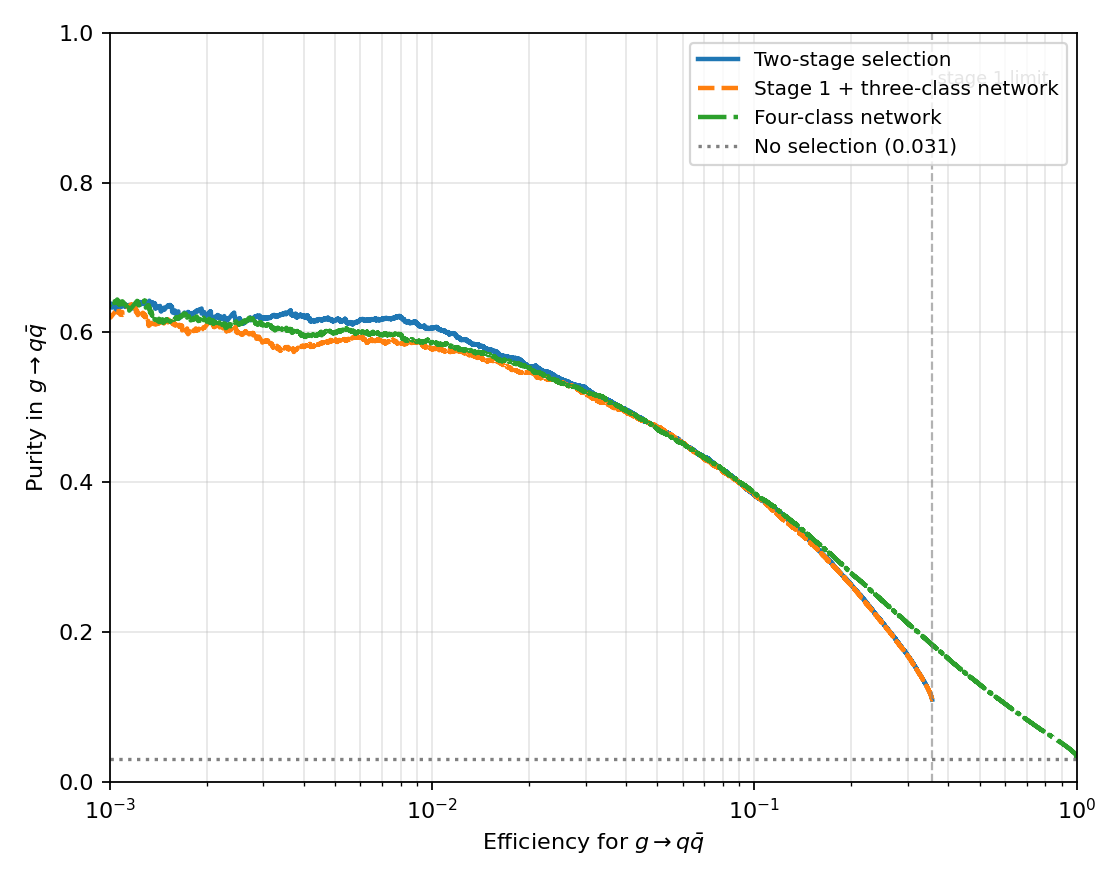
\includegraphics[width=0.75\textwidth]{figuras/purity_full_methods.png}
  \caption{Purity as a function of efficiency for the $g \to q\bar{q}$ channel,
  for the complete two-stage selection, for the first stage followed by the
  three-class network, and for the four-class network, applied to all labelled
  splittings of the simulated calibration sample. The vertical line marks the
  largest efficiency allowed by the requirement on the matched score, and the
  dotted line the purity before any selection.}
  \label{fig:purity-full}
\end{figure}

\begin{table}[htbp]
  \centering
  \caption{Purity of the complete selections at fixed efficiencies for the
  $g \to q\bar{q}$ channel, on all labelled splittings of the simulated
  calibration sample.}
  \label{tab:purity-full}
  \begin{tabular}{rccc}
    \toprule
    Efficiency (\%) & Two-stage & Stage 1 + three-class & Four-class \\
    \midrule
    $0.5$ & $0.622$ & $0.595$ & $0.606$ \\
    $1$   & $0.608$ & $0.579$ & $0.587$ \\
    $2$   & $0.556$ & $0.547$ & $0.553$ \\
    $5$   & $0.474$ & $0.475$ & $0.471$ \\
    $10$  & $0.383$ & $0.384$ & $0.386$ \\
    $20$  & $0.263$ & $0.262$ & $0.279$ \\
    $30$  & $0.168$ & $0.168$ & $0.211$ \\
    \bottomrule
  \end{tabular}
\end{table}

The three selections behave differently in different regions. At efficiencies
below about $2\%$, where the purity is highest, the two-stage selection reaches the
largest purity, by about $0.02$ to $0.03$ at an efficiency of $1\%$, a difference
of two to three times the statistical uncertainty of the purity. Between $5\%$ and
$10\%$ the three selections are equivalent. At larger efficiencies the four-class
network performs better, and it alone can exceed the efficiency of $35.7\%$ to
which the requirement on the matched score limits the other two. This is the
advantage of treating the rejection of the unmatched splittings and the
identification of the $g \to q\bar{q}$ channel in a single step.

However, for this measurement, the region of interest is the one with the highest purity
possible while keeping enough statistics. The
thresholds used in Section~\ref{sec:res-modulation} correspond to efficiencies
between about $28\%$ and $0.5\%$, and the most enriched samples lie below $5\%$,
where the two-stage selection performs best. The
two-stage selection is therefore retained for the measurement.

\section{Spin modulation as a function of the flavour selection}
\label{sec:res-modulation}

Finally, this section presents the main result of this work, the mean value
$\langle \cos 2\dpsi \rangle$ of the jets selected by the two-stage selection, as a
function of the threshold on the $g \to q\bar{q}$ score. Again, every jet is required 
to have a matched score greater than $0.8$ and the threshold on the second score goes
from $0.30$ to $0.60$ in steps of $0.05$. Because of statistics, the function does not
continue past $0.60$, since the number of selected jets becomes too small 
for the mean value to carry useful information, as discussed in
Section~\ref{sec:flavour-application}. Each threshold defines a sample increasingly
enriched in the $g \to q\bar{q}$ channel, and the evolution of the modulation along
this sequence of samples is the quantity of interest.

The purity computed for each threshold is that of a complete selection, determined 
in the simulation calibration sample. Its value depends on the treatment
of the jets that carry no channel label, for which no generator-level counterpart
was found or the generator-level declustering failed. These jets make up about
$31\%$ of the simulated jets with a valid $\dpsi$, and they are selected in data in
the same way as the others. Counting them as background gives a lower bound on the
purity, since some of them originate from genuine $g \to q\bar{q}$ splittings.
Excluding them gives the purity under the assumption that their composition is the
same as that of the labelled jets. Both values are quoted, and the true purity of
the selected samples lies between them.

Section~\ref{sec:res-mod-sim} presents the modulation in simulation, where the
composition of every selected sample is known.
Section~\ref{sec:res-mod-z} examines the kinematics of the selected splittings.
Section~\ref{sec:res-mod-data} compares the simulation with the collision data at
equal thresholds.

\subsection{Modulation in simulation}
\label{sec:res-mod-sim}

The mean value $\langle \cos 2\dpsi \rangle$ of the jets selected in the simulated
calibration sample is shown in Figure~\ref{fig:modulation-components}, as a function
of the threshold on the $g \to q\bar{q}$ score along with the obtained purity of the selection.
At the lowest measured threshold, the modulation of the selected jets is $-0.122 \pm 0.001$,
which is already stronger than measurement done on the inclusive sample of
Section~\ref{sec:res-inclusive}, $-0.083$, just by applying the matched score threshold.
As the threshold increases, the modulation becomes steadily more
negative and reaches $-0.266 \pm 0.016$ at $0.60$ while the purity goes from 
$0.18$ to between $0.48$ and $0.61$, depending on the treatment of the
jets without channel label. Thus, the modulation becomes more negative as the selected
samples are enriched in the $g \to q\bar{q}$ channel, as expected from the stronger
modulation of this channel found in Section~\ref{sec:res-labelling}.

\begin{figure}[htbp]
  \centering
  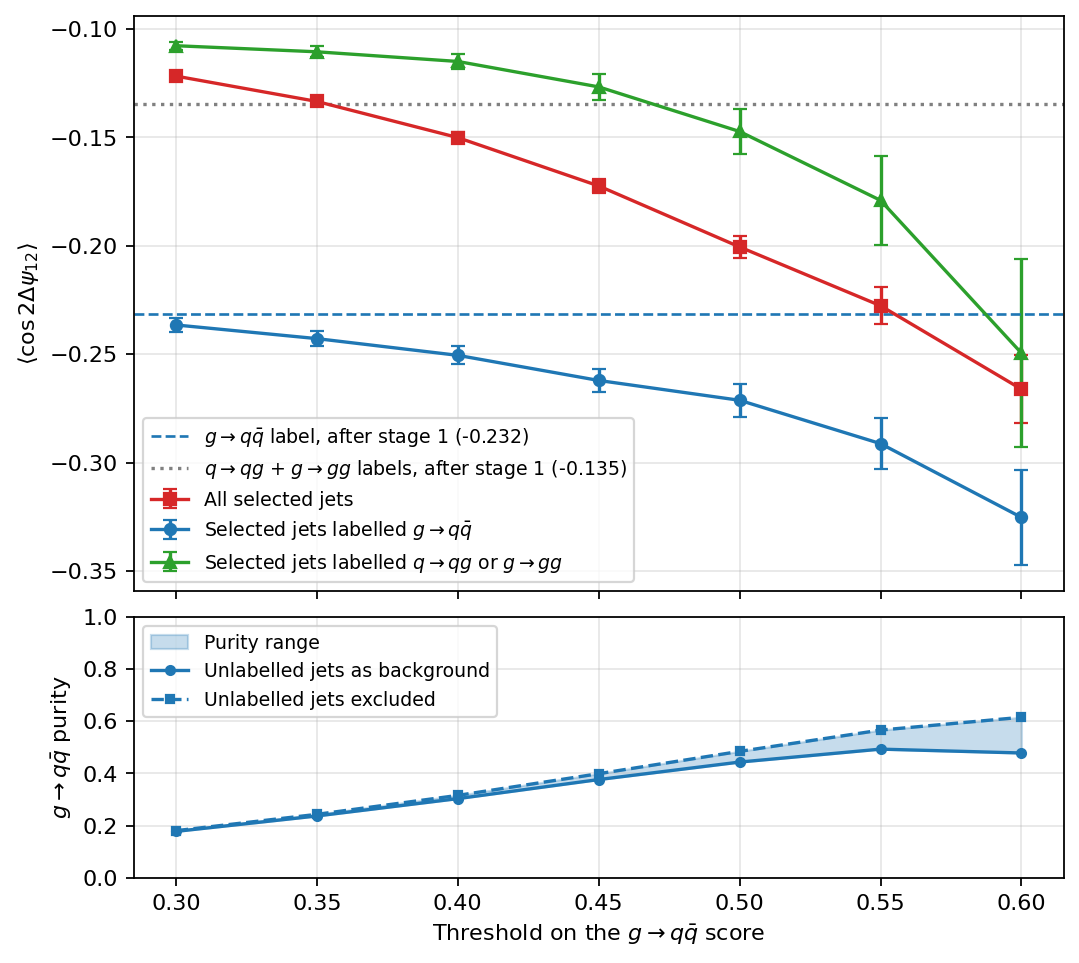
\includegraphics[width=0.7\textwidth]{figuras/modulation_components.png}
  \caption{Top: mean value $\langle \cos 2\dpsi \rangle$ of all jets selected by
  the two-stage selection in the simulated calibration sample, and of the selected
  jets labelled $g \to q\bar{q}$ and labelled $q \to qg$ or $g \to gg$, as a
  function of the threshold on the $g \to q\bar{q}$ score. All jets have a matched
  score above $0.8$. The horizontal lines show the mean values of the two classes
  with this requirement alone, without any threshold on the second score. Bottom:
  purity of the selected samples, with the jets without channel label counted as
  background and excluded, respectively.}
  \label{fig:modulation-components}
\end{figure}

The two purities coincide up to a threshold of about $0.45$, which shows that the
selected samples contain almost no jets without channel label at low thresholds.
The selection as a whole therefore strongly disfavours these jets, which make up
$31\%$ of the inclusive sample. At higher thresholds, however, the purities become
notably separated, and at a threshold of $0.60$ a fifth of the selected jets carry
no label. The tightest requirements thus retain proportionally more jets without a
generator-level counterpart, which causes the purity counting them as background
to saturate at about $0.5$.

The behaviour of the selection is further clarified by following the jets of the signal
and background classes separately. Among the jets passing the requirement on the
matched score, those labelled $g \to q\bar{q}$ have a mean value of
$-0.232 \pm 0.003$, and those labelled $q \to qg$ or $g \to gg$ a mean value of
$-0.135 \pm 0.001$. Within the selection, the jets labelled $g \to q\bar{q}$ become
steadily more negative as the threshold increases, from $-0.237 \pm 0.003$ at
$0.30$ to $-0.325 \pm 0.022$ at $0.60$. However, the background classes also become 
more negative as the threshold increases, from $-0.108 \pm 0.002$ at $0.30$ to $-0.249 \pm 0.043$
at $0.60$, and the decrease accelerates at the highest thresholds. At the lowest
thresholds their mean value lies above the reference of $-0.135$, which shows that
the first requirement on the second score removes background configurations with
a stronger than average modulation. The curve crosses the reference at a threshold
of about $0.47$, and at $0.60$ the background approaches the signal, although these
channels carry no or a slightly positive spin correlation. Therefore, 
the selection enriches the sample in the $g \to q\bar{q}$ channel and also
favours, at its tightest requirements, configurations in which the modulation 
is stronger whatever their channel.

Nevertheless, the difference between the two classes is still notable. Between
thresholds of $0.30$ and $0.50$, the jets labelled $g \to q\bar{q}$ lie between
$0.12$ and $0.14$ below the background selected at the same threshold. The
difference decreases only at the highest thresholds, to $0.11$ at $0.55$ and
$0.08 \pm 0.05$ at $0.60$, where both classes are dominated by the effect of the
selection. If the selection shifted the modulation of all channels by the same amount, this
shift would cancel in the difference between them, which would then remain
constant even as both classes become more negative. This is what is observed up to
a threshold of $0.50$. The stability of the difference therefore indicates that,
beyond the common effect of the selection, the $g \to q\bar{q}$ channel carries a
modulation of its own, about $0.13$ stronger than that of the background. At the
highest thresholds the difference decreases, which suggests that the effect of
the selection is no longer the same for all channels.

\subsection{Kinematics of the selected splittings}
\label{sec:res-mod-z}

The selection acts on the kinematics of each splittings as well as on their
flavour. The splitting function of equation~\eqref{eq:Pgq} favours symmetric
$g \to q\bar{q}$ splittings, in contrast with those of $g \to gg$ and $q \to qg$,
which are enhanced when one of the two products is soft. The distribution of the
momentum fraction $z_2$ of the second splitting is shown in the left panel of
Figure~\ref{fig:z-kinematics}. As one can notice, both classes rise towards $z_2 = 1/2$, since the
splitting of largest $\kt$ is selected in each sequence and $\kt$ grows with $z$.
However, their shapes are different. With jets below $z_2 \approx 0.3$ the channels
$q \to qg$ and $g \to gg$ are relatively more frequent, while above that those labelled
$g \to q\bar{q}$ are more frequent. The selection amplifies this effect, and with it,
at a threshold of $0.60$, almost no selected jet has $z_2 < 0.25$, and the distribution rises much
more steeply up to $z_2 = 1/2$. 

\begin{figure}[htbp]
  \centering
  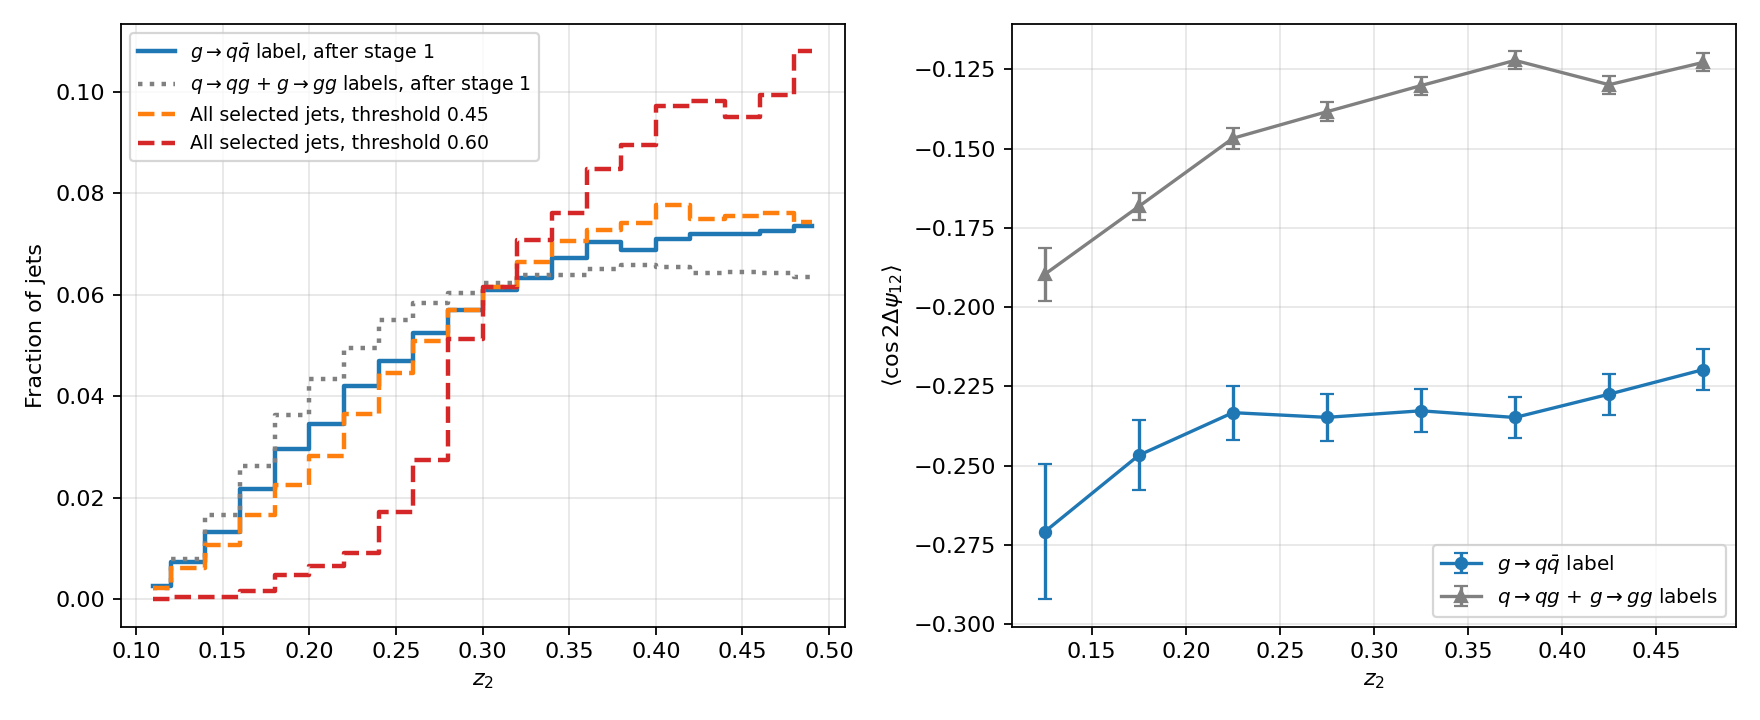
\includegraphics[width=\textwidth]{figuras/z_kinematics.png}
  \caption{Left: distribution of the momentum fraction $z_2$ of the second
  splitting for the jets labelled $g \to q\bar{q}$ and for those labelled
  $q \to qg$ or $g \to gg$ after the first stage, and for all jets selected at
  thresholds of $0.45$ and $0.60$, normalised to unit area. Right: mean value
  $\langle \cos 2\dpsi \rangle$ as a function of $z_2$ for the jets labelled
  $g \to q\bar{q}$ and for those labelled $q \to qg$ or $g \to gg$ after the first
  stage. All results are obtained on the simulated calibration sample.}
  \label{fig:z-kinematics}
\end{figure}

The dependence of the modulation on $z_2$ is shown in the right plot. For the background,
the modulation is most negative for asymmetric
splittings, $-0.19$ at $z_2 \approx 0.12$, and weakens to about $-0.12$ for
symmetric ones. These channels should carry no or a positive spin correlation, 
thus these reveals a component of the modulation that is not of spin
origin and is strongest for asymmetric splittings. For the jets labelled
$g \to q\bar{q}$ the modulation is instead nearly independent of $z_2$, at about
$-0.23$ over most of the range, whereas at leading order in the collinear limit
the spin correlation of this channel grows strongly towards symmetric
splittings~\cite{Karlberg_2021}. The difference between the two classes, which
removes the component common to both, grows from about $0.08$ for asymmetric
splittings to about $0.11$ for symmetric ones. It thus follows the expected
direction, but varies much less than predicted. This discrepancy is discussed in
Section~\ref{sec:res-discussion}.

These results explain part of the behaviour of Section~\ref{sec:res-mod-sim}. The
first requirements on the second score remove mainly background splittings with
low $z_2$, which carry the strongest modulation, so that the selected background
initially lies above its reference. The shift towards symmetric splittings cannot,
however, explain the strengthening of the modulation at the highest thresholds,
since symmetric splittings show a weaker modulation in the background and an
essentially unchanged one in the $g \to q\bar{q}$ class. Weighting the modulation
of each class by the distribution of $z_2$ of the jets selected at $0.60$ would
give about $-0.23$ for the $g \to q\bar{q}$ class and $-0.13$ for the background,
far from the observed values of $-0.325 \pm 0.022$ and $-0.249 \pm 0.043$. This
strengthening must therefore arise from other properties of the splittings to
which the classifier is sensitive, such as the momentum fraction of the first
splitting, the opening angles or the shapes of the branches, whose identification
is left for future work.

\subsection{Comparison with collision data}
\label{sec:res-mod-data}

The same selection procedure is applied to the collision data with the same networks
trained on simulation and the same requirements on both scores. The mean value
$\langle \cos 2\dpsi \rangle$ of the selected jets is compared with that of the
simulated calibration sample in Figure~\ref{fig:modulation-data}, however, 
the collision data is much smaller. At a threshold of $0.30$ it contains $2\,607$ jets, about $110$
times fewer than the $286\,380$ simulated ones, and only $162$, $50$ and $16$ jets
remain at $0.50$, $0.55$ and $0.60$. Therefore, the statistical uncertainty
of the data dominates the comparison at every threshold. Nevertheless,
the fraction of jets at low threshold are very similar between the two samples, by at most about $15\%$, 
which shows that the score distributions of data and simulation are close.

\begin{figure}[htbp]
  \centering
  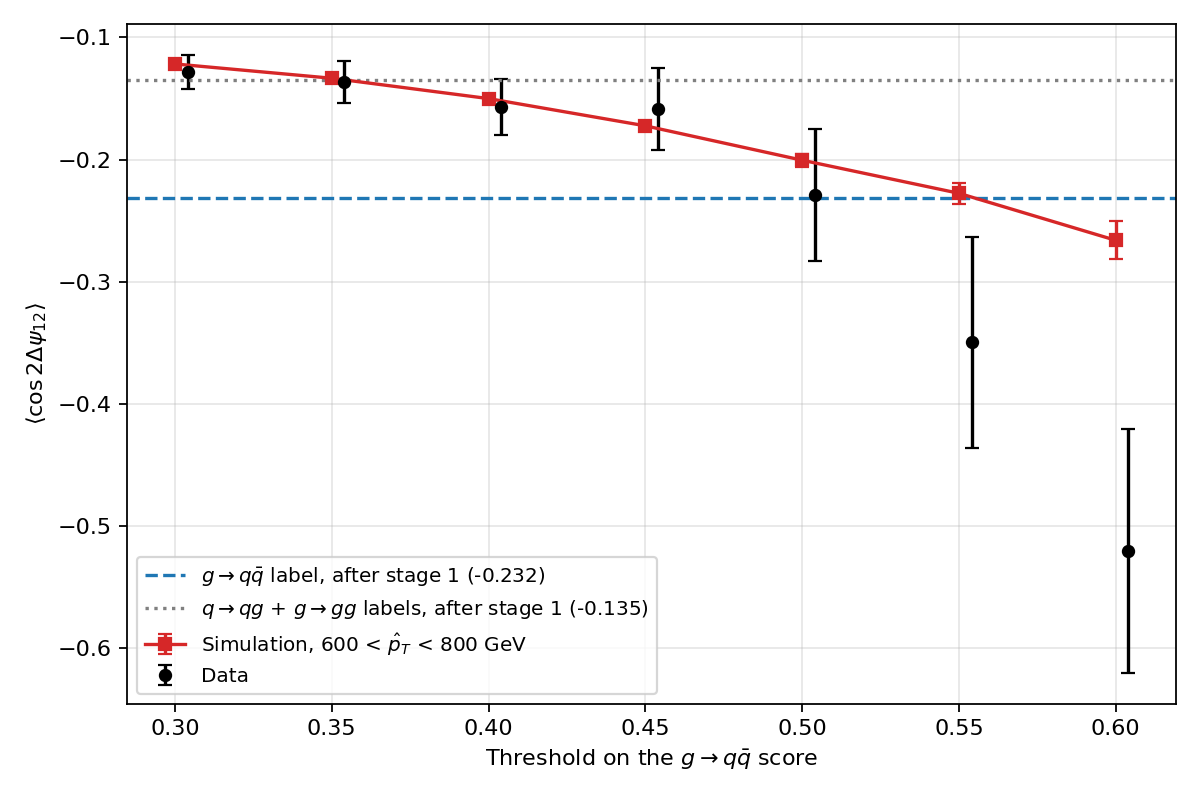
\includegraphics[width=0.7\textwidth]{figuras/modulation_threshold.png}
  \caption{Mean value $\langle \cos 2\dpsi \rangle$ of the jets selected by the
  two-stage selection as a function of the threshold on the $g \to q\bar{q}$
  score, in the collision data and in the simulated calibration sample. All jets
  have a matched score above $0.8$. The horizontal lines show the mean values in
  simulation of the jets labelled $g \to q\bar{q}$ and of those labelled
  $q \to qg$ or $g \to gg$ after this requirement alone. The data points are
  shifted slightly to the right for readability, and the error bars show the
  statistical uncertainties.}
  \label{fig:modulation-data}
\end{figure}

The quantitive comparison is restricted to thresholds up to $0.50$ since, in this range,
the data sample contains more than $150$ jets, and its statistical
uncertainty is at most about half of the difference of $0.097$ between the two
reference values. With thresholds above this value the uncertainty becomes comparable to this difference,
and the data can no longer distinguish a sample dominated by $g \to q\bar{q}$
splittings from one dominated by background.

Then, at thresholds below $0.5$, the mean values agree within less than one standard deviation, from
$-0.128 \pm 0.014$ in data and $-0.122 \pm 0.001$ in simulation at $0.30$ to
$-0.229 \pm 0.054$ and $-0.201 \pm 0.005$ at $0.50$. Thus, the modulation in data strenghtens
with the threshold, just like in simulation. Since the selected samples are
grouped together, the jets selected at $0.50$ are also part of the sample at $0.30$, and the
uncertainty of the change between the two thresholds is approximately
$\sqrt{\sigma_{0.50}^2 - \sigma_{0.30}^2}$, smaller than the combination of the two
uncertainties. Between $0.30$ and $0.50$ the mean value in data decreases by
$0.101 \pm 0.052$, compared with $0.079$ in simulation. Therefore, the strengthening is
seen in data with a significance of about two standard deviations.

However, above the threshold of $0.50$, the data lies below the simulation, by $1.4$ standard deviations at
$0.55$ and by $2.5$ at $0.60$, where the mean value reaches $-0.52 \pm 0.10$. These
two points rest on very few jets and are strongly correlated. The $16$ jets
selected at $0.60$ are also part of the $50$ selected at $0.55$, and the remaining
$34$ jets, with scores between $0.55$ and $0.60$, have a mean value of about
$-0.27$, in agreement with the simulation. The deviation at both thresholds
therefore comes mostly from the $16$ jets of highest score. With so few jets the
Gaussian approximation of the uncertainty is itself unreliable, and the central
value at $0.60$ even lies beyond $-1/2$, the most negative value allowed by a
modulation of the form of equation~\eqref{eq:dpsi-modulation}. This illustrates the
size of the statistical fluctuations at these thresholds, and a deviation of this
kind in the last of several correlated points is not evidence of a disagreement
with simulation.

Within the precision of the data, it is possible to say that it describes both
the response of the selection and the modulation of the selected jets. However this
agreement does not establish the presence of spin correlation in data, since 
part of the strengthening of the modulation in simulation is common to all
channels and is induced by the selection itself, as shown in
Section~\ref{sec:res-mod-sim}, and no simulated sample without spin correlations is
available to isolate the contribution of spin origin. These points are discussed
in Section~\ref{sec:res-discussion}.

\section{Three-point energy correlator}
\label{sec:res-eeec}

The three-point energy correlator of Section \ref{sec:eeec-impl} gives a second probe of
the spin correlations, built directly from jet constituents and independent of the declustering.
Its distribution in the azimuthal angle $\psi$ is computed over
all triplets of constituents inside the window of equation \eqref{eq:eeec-window}, each
with the weight of equation \eqref{eq:eeec-weight}, and normalised to unit area over
$(-\pi,\pi]$. Its modulation is summarised by the weighted mean

\begin{equation}
  \langle \cos 2\psi \rangle =
  \frac{\sum_{\text{jets}} \sum_{abc} w_{abc} \cos 2\psi_{abc}}
       {\sum_{\text{jets}} \sum_{abc} w_{abc}} ,
  \label{eq:eeec-mean}
\end{equation}

which is related to the coefficients of a modulation of the form of
equation \eqref{eq:dpsi-modulation} by $a_2/a_0 = 2\langle \cos 2\psi \rangle$, as for
$\dpsi$. The constituents of a jet share elements with one another and are therefore 
not independent, thus, statistical uncertainties are calculated by treating the jets 
as the independent units. Since the simulated calibration dataset is much larger than 
the collision dataset, the distributions of all jets
are obtained from the first $5 \times 10^{5}$ events which makes 
the statistical uncertainty much smaller than that of the data while the latter uses 
all selected events. For the labelled classes in the simulated calibration dataset,
all events were used.

The distribution of all jets is shown in the left panel of Figure \ref{fig:eeec-distributions}.
This distribution reveals a clear modulation, symmetric under $\psi \to -\psi$ as 
expected from parity invariance, with maxima at $\psi = 0$ and $\pm\pi$ and minima at $\pm\pi/2$.
The mean values obtained are $+0.020 \pm 0.001$ in data and
$+0.019 \pm 0.001$ in simulation, which is equivalent to $a_2/a_0 \approx +0.04$,
and the ratio of data to simulation is compatible with unity within about $2\%$ in
every bin. The shape is closer to a single $\cos 2\psi$ harmonic, with, however,
a minima somewhat deeper than this harmonic would produce, as it is possible to
see when comparing to the red dashed line. With this, the obtained distribution 
has positive sign and thus it is opposite to that of the inclusive $\dpsi$
distribution of Section~\ref{sec:res-inclusive}, and about four times smaller in
magnitude.

\begin{figure}[htbp]
  \centering
  \begin{minipage}{0.49\textwidth}
    \centering
    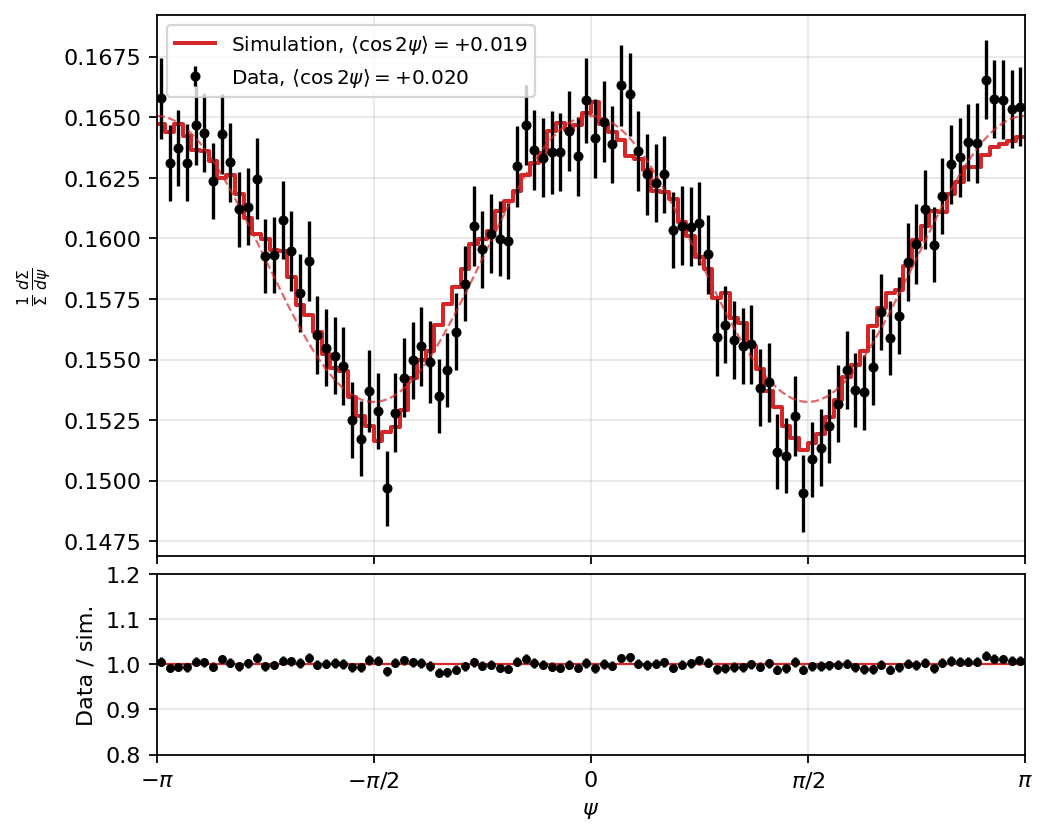
\includegraphics[width=\textwidth]{figuras/eeec_inclusive.png}
  \end{minipage}\hfill
  \begin{minipage}{0.49\textwidth}
    \centering
    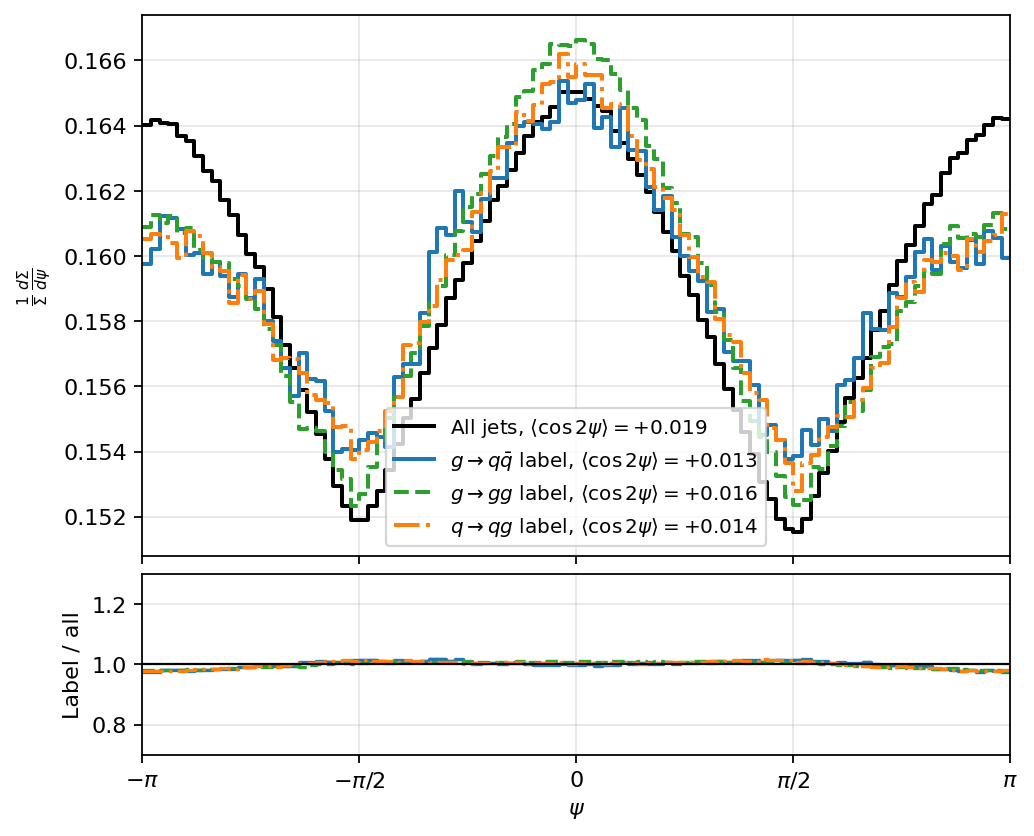
\includegraphics[width=\textwidth]{figuras/eeec_labels.png}
  \end{minipage}
  \caption{Distribution of the azimuthal angle $\psi$ of the three-point energy
  correlator, normalised to unit area. The left panel compares all jets in the
  collision data and in the simulated calibration sample, with the ratio of data
  to simulation in the lower panel. The right panel shows the simulated jets
  labelled $g \to q\bar{q}$, $g \to gg$ and $q \to qg$ together with all simulated
  jets, with the ratio of each class to all jets in the lower panel. The dashed
  line in the left panel is the pure $\cos 2\psi$ modulation with the mean value
  of the simulation.}
  \label{fig:eeec-distributions}
\end{figure}

The right panel of Figure \ref{fig:eeec-distributions} shows the seperation by channel label,
and demonstrates almost no dependence on the channel. All channels demonstrate a positive 
modulation of close size. The mean value is $+0.0125 \pm 0.0006$ for the
jets labelled $g \to q\bar{q}$, $+0.0136 \pm 0.0004$ for $q \to qg$ and
$+0.0161 \pm 0.0002$ for $g \to gg$, and the distributions of the three classes
differ from that of all jets by at most about $3\%$ in every bin. The jets of
the $g \to q\bar{q}$ channel have the weakest positive modulation and 
they differ from the other classes by less than $0.004$. In comparison with the
$\dpsi$ modulation, the same label has a much negative modulation, as shown in Section~\ref{sec:res-labelling}.
This main difference between the observables happens because of how they are built. The channel
label corresponds to the second splitting of the Lund declustering, while the three-point energy
correlator sums over every triplet inside a fixed angular window, most of which do not
resolve that splitting. Therefore, a jet with a labelled channel of $g \to q\bar{q}$
mainly contributes to the correlator through triplets unrelated to its $g \to q\bar{q}$ splitting.
The mean value of all jets, $+0.019 \pm 0.001$, is larger than that of
every labelled class because it is dominated by the unmatched jets and by those
without a label. These make up almost $90\%$ of the jets and have mean values of
$+0.0200$ and $+0.0196$.

The labelled channels also show a feature that is much weaker in the sample with all jets. 
Their maximum at $\psi = \pm\pi$ is about $3\%$ lower than that at
$\psi = 0$, which corresponds to a term in $\cos\psi$. Exchanging the two closest
constituents $a$ and $b$ reverses the normal $\hat{n}_1$ of
equation \eqref{eq:eeec-normals} and shifts $\psi$ by $\pi$. Therefore, the distinction between
$\psi = 0$ and $\psi = \pm\pi$ depends on which of the two is taken as
$a$, here the one stored first. A term of this kind does not have the period $\pi$
of the spin correlation and does not contribute to $\langle \cos 2\psi \rangle$.

The three-point energy correlator of the jets selected by the flavour selection procedure are shown
in Figure \ref{fig:eeec-threshold} as a function of the threshold. After passing the first 
selection stage and the requirement of having a matched score above $0.8$, 
the jets labelled $g \to q\bar{q}$ and the
background have mean values of $+0.010$ and $+0.012$, which differ by only $0.002$,
compared with about $0.10$ for $\dpsi$. Therefore, using the networks to enrich the samples
with the $g \to q\bar{q}$ label can barely change the correlator. Nevertheless, in simulation
the mean value decreases steadily with the threshold, from about
$+0.014$ at $0.30$ to about $+0.001$ at $0.60$, and it lies outside the range
spanned by the two references at both ends. Its size, about $0.013$, is however an order of
magnitude smaller than the corresponding change of $\dpsi$ seen in Section~\ref{sec:res-mod-sim}.
The data follow the
simulation. Up to a threshold of $0.50$, the range retained in
Section~\ref{sec:res-mod-data}, they differ from it by at most about $1.3$ standard
deviations, from $+0.017 \pm 0.004$ against $+0.014$ at $0.30$ to
$-0.007 \pm 0.021$ against $+0.010$ at $0.50$. Above this threshold the
uncertainty of the data exceeds the whole variation of the simulation.

\begin{figure}[htbp]
  \centering
  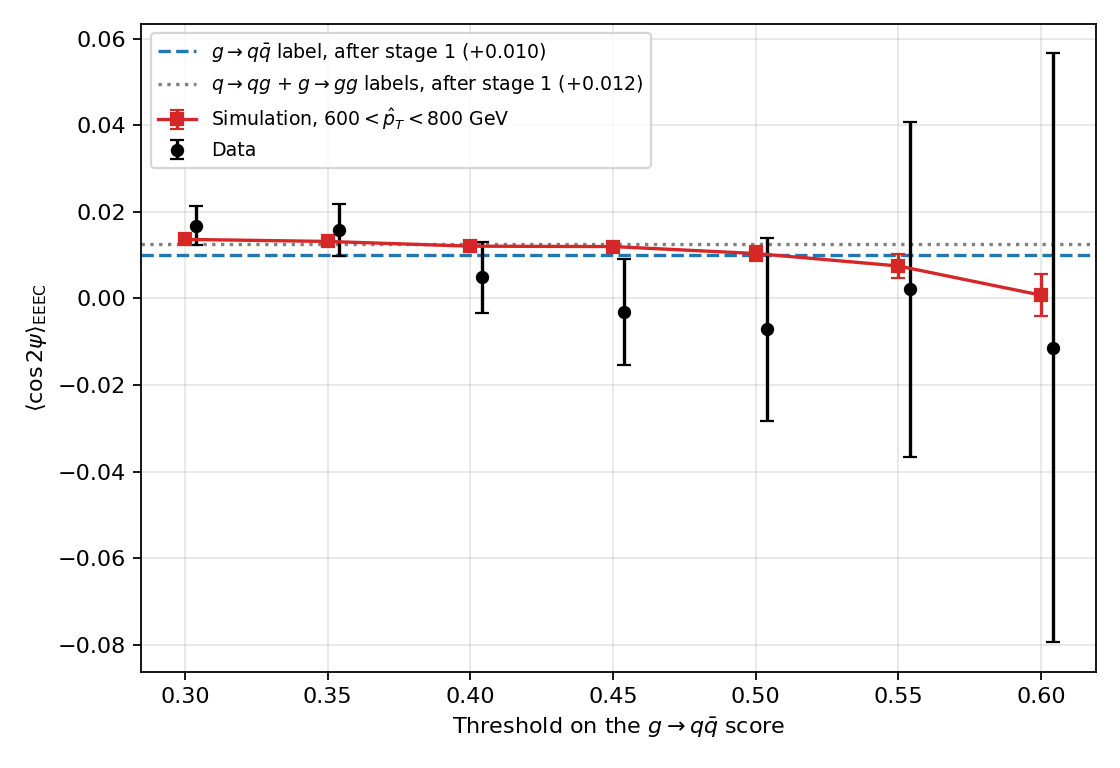
\includegraphics[width=0.6\textwidth]{figuras/eeec_threshold.png}
  \caption{Mean value $\langle \cos 2\psi \rangle$ of the three-point energy
  correlator of the jets selected by the two-stage selection as a function of the
  threshold on the $g \to q\bar{q}$ score, in the collision data and in the
  simulated calibration sample. All jets have a matched score above $0.8$. The
  horizontal lines show the mean values in simulation of the jets labelled
  $g \to q\bar{q}$ and of those labelled $q \to qg$ or $g \to gg$ after this
  requirement alone. The data points are shifted slightly to the right for
  readability, and the error bars show the statistical uncertainties.}
  \label{fig:eeec-threshold}
\end{figure}

Thus, the three-point energy correlator shows a modulation that the simulation follows the
collision data, although with a positive sign, nearly insensitive to the channel
labelling of the Lund declustering, and only weakly affected by a flavour selection
built on the declustering. It does not reproduce the strong negative modulation
associated with $g \to q\bar{q}$ splittings in the $\dpsi$ observable. These
results are compared with the theoretical expectations of
\cite{Karlberg_2021} in Section~\ref{sec:res-discussion}.

\section{Discussion}
\label{sec:res-discussion}

The previous sections presented the computation of the two spin-sensitive
observables in collision data and simulation, before and after flavour selection.
This section interprets these results, compares them with the theoretical
expectations of \cite{Karlberg_2021}, obtained at second order in the
collinear limit for electron-positron collisions, and with the CMS
measurement~\cite{CMS:2026jnt}, which observed the spin correlations in
$g \to q\bar{q}$ splittings with an analysis similar to the present one. 

The discussion is organised in four parts. Section~\ref{sec:disc-theory} examines
whether the observed modulations have the properties expected from spin
correlations. Section~\ref{sec:disc-selection} discusses the effect of the flavour
selection on the modulation, and Section~\ref{sec:disc-cms} the comparison with
the CMS measurement. Section~\ref{sec:disc-limits} summarises the limitations of
the analysis that follow from these comparisons.

\subsection{Comparison with theoretical expectations}
\label{sec:disc-theory}

In simulation, the jets labelled as $g \to q\bar{q}$ revealed the most negative modulation,
$\langle \cos 2\dpsi \rangle = -0.167 \pm 0.002$, but with half the magnitude of the collinear prediction of, $-0.31$. 
A weaker modulation is, although, expected 
for several reasons. The IFN label is a flavour proxy and does not
coincide splitting by splitting with the vertex of the parton shower.
The observable was built from reconstructed, after hadronisation and detector effects.
The prediction also refers to quark-initiated jets in electron-positron collisions. This
work is done in proton-proton collisions and a large fraction of the jets are initiated by gluons,
which the intermediate gluon is produced in a
$g \to gg$ splitting with a different degree of polarisation, so no prediction
specific to proton--proton collisions is available for $\dpsi$.

A larger deviation appears on the classes which little or no spin correlation is expected.
The jets, with labels $g \to gg$ and $q \to qg$, have mean values of
$-0.077$ and $-0.091$, where the predictions are $+0.025$ and zero, and the
unmatched jets have $-0.059$. For all jets together, the inclusive value of
$-0.083$ in simulation and $-0.078$ in data compares with a prediction of about
$-0.013$. Thus, a negative component of the modulation is present on each channel.
Two of its properties are visible in the results.
It depends strongly on the kinematics of the second splitting and is largest for
asymmetric splittings, as shown in Section~\ref{sec:res-mod-z}. It is also
accompanied by higher harmonics in the inclusive distribution of
Section~\ref{sec:res-inclusive}, whereas a collinear spin correlation at this
order contributes only a $\cos 2\dpsi$ term. Both properties suggest an origin in
the kinematics of the declustering rather than in the spin of the intermediate
gluon. The simulation reproduces this component in data, so it is described by the
generator and the detector simulation, but its origin is not identified in this
work. Its dominance is consistent with the CMS measurement, in which switching off the
spin correlations in \textsc{Pythia}~8 changes the inclusive distribution of
$\dpsi$ by only about $0.5\%$~\cite{CMS:2026jnt}.

Since this component is common to all classes, the difference between the
$g \to q\bar{q}$ class and the background is the quantity closest to the spin
correlation of the $g \to q\bar{q}$ channel. Before any selection it amounts to
$0.086$, from $-0.167$ and $-0.081$, and after the first stage of the selection to
$0.097$, from $-0.232$ and $-0.135$. Both values are less than a third of the
difference of about $0.33$ between the predictions for the $g \to q\bar{q}$ and
$g \to gg$ channels. Also, the dependence of this difference on $z_2$ is much weaker
than expected. At leading order, the azimuthal dependence of the
$g \to q\bar{q}$ splitting of a linearly polarised gluon is proportional to
$1 - 2z(1-z) - 2z(1-z)\cos 2\phi$, so that its analysing power,
$2z(1-z)/[1 - 2z(1-z)]$, grows from $0.22$ at $z_2 = 0.1$ to $1$ at $z_2 = 1/2$.
The difference computed instead grows from about $0.08$ below $z_2 = 0.2$ to about
$0.10$ above $z_2 = 0.3$. This may be either the non-spin
component does not cancel completely in the difference, or the spin correlation
is strongly diluted at reconstruction level because of the smearing of $z_2$,
the cases where the reconstructed splitting does not correspond to the
generator-level one, and by those in which
the label does not correspond to the channel of the shower. 
The two effects cannot be separated without a reference in
which the spin correlations are absent, as discussed in
Section~\ref{sec:disc-cms}.

The three-point energy correlator departs further from the expectations. 
For quark-initiated jets in electron-positron collisions, In \cite{Karlberg_2021} predicts mean
values $\langle \cos 2\psi \rangle$ of about $-0.18$ for the $g \to q\bar{q}$
channel, $+0.013$ for $g \to gg$ and $-0.004$ for all jets together. The result 
obtained here in this work is positive, $+0.0186 \pm 0.0001$ in simulation and
$+0.0200 \pm 0.0012$ in data, and it depends little on the channel label. The jets
labelled $g \to q\bar{q}$, with $+0.0125 \pm 0.0006$, differ from those labelled
$g \to gg$ by only $0.004$. The weak dependence on the label follows may come from 
the construction of the correlator, which sums over all triplets inside a fixed window
and thus not tied to the second splitting of the declustering, as
discussed in Section~\ref{sec:res-eeec}. The positive sign is not explained here, but
it may reflect the larger fraction of gluon-initiated jets at a hadron collider,
whose $g \to gg$ splittings contribute positively, the transposition of the
angular window from electron-positron collisions to the $(\eta,\phi)$ plane, or a
non-spin component of the same kind as the one found for $\dpsi$. However,
the present work does not discriminate between these possibilities.

\subsection{Effect of the flavour selection}
\label{sec:disc-selection}

The flavour selection developed in this work strengthens the modulation of the selected jets from
$-0.122$ at a threshold of $0.30$ to $-0.266$ at $0.60$, while the purity rises
from about $0.18$ to between $0.48$ and $0.62$. If the selection only changed the proportions
of the channels, the jets of each class would keep the modulation they have after
the first stage, $-0.232$ for the $g \to q\bar{q}$ class and $-0.135$ for the
background, and the mean value of the labelled jets would lie between these two
values. So, at a threshold of $0.60$, where the observed purity was at most $0.62$, 
such a mixture would give a modulation of $-0.19$. However, at this threshold,
the labelled jets selected have instead a mean value of about $-0.30$, more negative than the reference of
the $g \to q\bar{q}$ class itself.

Thus, the modulation of each class changes with the threshold. The jets labelled
$g \to q\bar{q}$ become more negative, from $-0.237$ to $-0.325$, and the jets
labelled $q \to qg$ or $g \to gg$ even more so, from $-0.108$ to $-0.249$,
even though their label does not change. There are two possible explanations, and
they are not exclusive. The first one is that the classifier, which does not use $\dpsi$ as an
input, selects configurations in which the non-spin component of the modulation 
identified in Section~\ref{sec:disc-theory} is stronger, through features
correlated with it. Part of this effect is explained by the momentum fraction of
the second splitting, as shown in Section~\ref{sec:res-mod-z}. The second one 
is that the shift reflects the limitations of the IFN label. The label does not
coincide splitting by splitting with the vertex of the parton shower, and the classifier,
trained on the substructure of the branches, may recognise real
$g \to q\bar{q}$ splittings better than the label does. At high thresholds, the jets 
with the label of $g \to q\bar{q}$ would then mostly be those in which the label is
correct, and the jets labelled as background would increasingly be
$g \to q\bar{q}$ splittings that the label assigns to another channel. Thus,
both would carry a stronger spin correlation, and the true purity would be
higher than the purity defined by the IFN label. The mean value of the
jets labelled $g \to q\bar{q}$ at the highest threshold, $-0.325 \pm 0.022$, close
to the prediction of $-0.31$, is consistent with this interpretation. As argued in
Section~\ref{sec:disc-theory}, however, the negative modulation of the background
before any selection cannot be attributed to such splittings.

The difference between the two classes stays close to $0.13$ from a threshold of
$0.30$ up to $0.50$, and decreases to $0.076 \pm 0.049$ at $0.60$. According to the
first explanation, the common shift cancels in this difference, and, according to the second one,
decrease at the highest thresholds would reflect the growing fraction of genuine
$g \to q\bar{q}$ splittings among the jets labelled as background, although it is
not significant within the statistical uncertainties. Unfortunately, the two explanations
cannot be separated with the samples available in this work. They would differ only on
a sample where no spin correlations are present, in which the first would still produce 
a shift and the second would not, and in the dependence of the additional modulation on
$z_2$, which should grow towards symmetric splittings if it is of spin origin. In
either case, the mean value of the selected sample combines the enrichment in
$g \to q\bar{q}$ splittings with effects that cannot be separated from it in data.
For this reason, the result is presented as a function of the threshold, and not instead 
as a function of the purity. A linear extrapolation of the modulation
to a purity of one would assume that the modulations of the signal and of the
background do not depend on the threshold, and the simulation shows that this
assumption does not hold.

The comparison with the collision data is subject to the same limitation. Between thresholds of
$0.30$ and $0.50$ the modulation in data strengthens by $0.101 \pm 0.052$,
compared with $0.079$ in simulation. Therefore, the collision data follows the simulation,
but this agreement holds whichever of the two
explanations applies, and it does not distinguish between them.

The energy correlator also behaves in a similar way. Its mean value decreases with the
threshold by about $0.013$ for all selected jets and by a similar amount for those
labelled $g \to q\bar{q}$, from $+0.0093$ to $-0.0017$, although the two labelled
references after the first stage differ by only $0.0025$. Therefore,
the selection changes the correlator
mainly through properties of the selected jets other than their label.

\subsection{Comparison with the CMS measurement}
\label{sec:disc-cms}

The CMS measurement used $34.7$~fb$^{-1}$ of proton-proton collisions recorded in
2022 at $\sqrt{s} = 13.6$~TeV~\cite{CMS:2026jnt}. The distribution of $\dpsi$ in
the selected jets was compared with the predictions of \textsc{Pythia}~8 and
\textsc{Herwig}~7, each with and without the angular correlations induced by the
gluon spin. The hypothesis without correlations is disfavoured with an observed
significance of $6.8$ standard deviations, for an expected $8.1$, while the data
differ from the hypothesis with correlations by $1.9$ standard deviations and
favour a slightly weaker modulation than predicted. Its strategy is very close to the
one followed here.
The composition of the simulated samples is very similar, as shown in
Section~\ref{sec:res-labelling}. The purity reached by CMS, $38\%$ for a score
above $0.6$ in its four-class network, is also of the same order as the purities
obtained here, from $0.38$-$0.40$ at a threshold of $0.45$ to $0.44$-$0.49$ at
$0.50$, although the two analyses define the purity with different matching
criteria.

Nevertheless the two analysis differ in several aspects. CMS reconstructs jets
using the PUPPI algorithm for pileup mitigation, while the jets in this work 
are corrected with charged-hadron subtraction, and it applies the requirements on
the constituents and on the second subjet discussed in
Section~\ref{sec:sys-choices}. CMS' classifier has four classes and is trained on
the \textsc{Herwig}~7 sample without spin correlations, so that it cannot exploit
the modulation itself. Here the selection is performed in two stages and trained
on a \textsc{Pythia}~8 sample. However, the four-class network studied as an
alternative in Section~\ref{sec:res-performance} performs comparably to the
two-stage selection, so that the choice of architecture is not expected to be the
main difference between the two results.

The decisive difference lies in the predictions against which the data are
compared. In CMS, the predictions with and without spin correlations are processed
through the same selection, so that every effect of the selection that does not
originate from the spin is present in both and cancels in their comparison. These
predictions also show how small the spin-induced part of the modulation is. In
\textsc{Pythia}~8, switching off the correlations changes the inclusive
distribution by only about $0.5\%$, and the distribution of the selected
$g \to q\bar{q}$ category by at most $12\%$~\cite{CMS:2026jnt}. This is consistent
with the large non-spin component found in Section~\ref{sec:disc-theory}, which
the selection does not remove. The same comparison would also separate the two
explanations of Section~\ref{sec:disc-selection}, since a shift caused by the
selection of the non-spin component would persist without spin correlations,
whereas a shift caused by genuine $g \to q\bar{q}$ splittings assigned to other
channels would disappear.

In \textsc{Pythia}~8 the correlations are included as an average modulation of the
angle between the production and splitting planes of the
gluon~\cite{CMS:2026jnt}, and the nominal sample used here therefore corresponds
to a prediction with correlations. The agreement between data and simulation found
in Section~\ref{sec:res-mod-data} is thus consistent with the CMS observation that
the data agree with \textsc{Pythia}~8 with correlations. No sample without spin
correlations is available among the CMS Open Data simulations of the period
studied here, however, so this agreement cannot be turned into a statement on the
presence of spin correlations in the data. A numerical comparison of the
modulation itself is not possible either, since CMS presents the distribution of
$\dpsi$, at detector and at particle level, but not its mean value
$\langle \cos 2\dpsi \rangle$. The present analysis thus reproduces the strategy of
the CMS measurement with public data from an earlier period, but cannot by itself
reach its conclusion. What it adds is a decomposition of the modulation by channel
class in simulation, which shows how the flavour selection acts on each class and
why the modulation of the selected samples cannot be interpreted as that of the
$g \to q\bar{q}$ channel alone.

\subsection{Limitations}
\label{sec:disc-limits}

The main limitations of this analysis come from the preceding subsections. The 
most important is the absence of a simulation without spin correlations. The simulation
used here includes the approximate treatment of the correlations of
\textsc{Pythia}~8, and the CMS measurement shows that the spin-induced part of the
modulation is small compared with the non-spin component. Without a reference using 
the same selection, but with
the correlations are turned off, the two components cannot be separated, and neither can the two
explanations of the effect of the selection discussed in
Section \ref{sec:disc-selection}.

This analysis also relies on a single generator. \textsc{Pythia}~8 with the CP5
tune is used for the training of the classifier, for the calibration of the
selection, for the determination of the purity and for the comparison with data.
The dependence of the composition and of the purity on the description of the
parton shower and of the hadronisation is therefore not tested, as discussed in
Section~\ref{sec:sys-purity}. This dependence is likely to be relevant, since
\textsc{Pythia}~8 and \textsc{Herwig}~7 treat the spin correlations differently
and predict different strengths of the modulation \cite{CMS:2026jnt}.

The computed purity is defined through the IFN label, which is a flavour proxy
assigned through an angular matching. About $31\%$ of the simulated jets carry no label,
which is why the purity is quoted in an interval, and the true fractions
of $g \to q\bar{q}$ splittings in the selected samples may differ from the labelled
one, as discussed in Section~\ref{sec:disc-selection}.

The collision data correspond to a single period of data taking, with about
$4.6 \times 10^{4}$ jets with a valid $\dpsi$. Their statistical precision limits
the comparison with simulation to thresholds up to $0.50$, and it is insufficient
to resolve differences of the size expected between predictions with and without
spin correlations. All results are also obtained at detector level, without
correction for the resolution and acceptance of the detector, so their comparison
with theoretical predictions is only qualitative. Finally, only statistical
uncertainties are given. The systematic sources of Section~\ref{sec:systematic}
are not propagated, and the analysis choices that differ from the CMS
measurement, discussed in Section~\ref{sec:sys-choices}, are not varied.

Within these limitations, the analysis shows that the full chain, from the
released data to a flavour-enriched measurement of the modulation, can be carried
out with public data and tools. It also shows that the simulation describes the
data well in the observables central to this work, namely the plane
$(z_1, z_2)$, the modulation as a function of the threshold and the energy
correlator. The extensions needed to turn this agreement into a statement on the
presence of spin correlations are discussed in Chapter~\ref{cap:conclusoes}.